\documentclass[10pt,a4paper,twocolumn]{article}

% ── Page ────────────────────────────────────────────────────
\usepackage[a4paper, left=1.7cm, right=1.7cm, top=2.3cm, bottom=2.0cm,
            headheight=18pt, headsep=10pt, columnsep=6mm]{geometry}

% ── Fonts: Times-like text and maths, as in most journals ───
\usepackage[T1]{fontenc}
\usepackage[utf8]{inputenc}
\usepackage{newtxtext}
\usepackage{newtxmath}
\usepackage{microtype}

% ── Content ─────────────────────────────────────────────────
\usepackage{amsmath}
\usepackage{graphicx}
\usepackage[dvipsnames]{xcolor}
\usepackage{booktabs}
\usepackage{array}
\usepackage{tabularx}
\usepackage{enumitem}
\usepackage{listings}
\usepackage{textcomp}
\usepackage[round]{natbib}
\usepackage[font=small, labelfont=bf, labelsep=period, skip=4pt]{caption}
\usepackage{titlesec}
\usepackage{fancyhdr}
\usepackage{lastpage}
\usepackage[colorlinks=true, linkcolor=MidnightBlue, citecolor=MidnightBlue,
            urlcolor=MidnightBlue, bookmarks=true]{hyperref}

\usepackage{xurl}                          % long URLs break across lines
\usepackage{orcidlink}

% ── Journal-style headings: numbered, serif, restrained ─────
\titleformat{\section}{\normalfont\large\bfseries}{\thesection}{0.6em}{}
\titleformat{\subsection}{\normalfont\normalsize\bfseries}{\thesubsection}{0.5em}{}
\titleformat{\subsubsection}{\normalfont\normalsize\itshape}{\thesubsubsection}{0.5em}{}
\titlespacing*{\section}{0pt}{1.4ex plus 0.6ex}{0.7ex}
\titlespacing*{\subsection}{0pt}{1.1ex plus 0.4ex}{0.5ex}
\setlength{\parindent}{1em}
\setlength{\parskip}{0pt}
\raggedbottom                               % no stretched gaps to fill columns
\setlist{leftmargin=*, itemsep=0.2em, topsep=0.3em}

% ── Running header: name and version left, logo right ───────
\newcommand{\headerlogo}{
\includegraphics[height=10pt]{fermium_logo_header_black.png}}
\newcommand{\docversion}{Technical documentation v2.0}
\pagestyle{fancy}
\fancyhf{}
\fancyhead[L]{\footnotesize Fermium Hazard Mapper \textperiodcentered{} \href{https://fermium.systems/hazmapper}{fermium.systems/hazmapper}}
\fancyhead[R]{\headerlogo}
\fancyfoot[C]{\footnotesize \thepage\ of \pageref{LastPage}}
\renewcommand{\headrulewidth}{0pt}
\fancypagestyle{firstpage}{\fancyhf{}%
  \fancyhead[R]{\headerlogo}%
  \fancyfoot[C]{\footnotesize \thepage\ of \pageref{LastPage}}%
  \renewcommand{\headrulewidth}{0pt}}
\fancypagestyle{plain}{\fancyhf{}%
  \fancyhead[L]{\footnotesize Fermium Hazard Mapper \textperiodcentered{} \href{https://fermium.systems/hazmapper}{fermium.systems/hazmapper}}%
  \fancyhead[R]{\headerlogo}%
  \fancyfoot[C]{\footnotesize \thepage\ of \pageref{LastPage}}%
  \renewcommand{\headrulewidth}{0pt}}

% ── Code listings fit a single column ──────────────────────
\lstset{basicstyle=\footnotesize\ttfamily, breaklines=true,
        columns=fullflexible, frame=tb, framerule=0.3pt,
        aboveskip=0.5em, belowskip=0.5em}

% ── Monospace that breaks at underscores ───────────────────
\makeatletter
\let\orig@texttt\texttt
\renewcommand{\texttt}[1]{%
  \ifmmode\text{\orig@texttt{#1}}\else
  \begingroup\ttfamily\def\_{\textunderscore\allowbreak}#1\endgroup\fi}
\makeatother
\newcommand{\fileref}[1]{\texttt{#1}}

% Generated by docs/build_numbers.py — do not edit by hand.
% Built 2026-09-23T04:26:15+00:00
%
% Any figure the pipeline did not produce renders as \todo{missing},
% so a gap is visible in the PDF rather than filled from memory.
\providecommand{\todo}[1]{\textbf{[TODO: #1]}}

% ---- rangpur_rajshahi ----
\newcommand{\RRAssets}{37,012}
\newcommand{\RRLabelRate}{4.8}
\newcommand{\RRValAUC}{0.886}
\newcommand{\RRValAP}{0.454}
\newcommand{\RRValBrier}{0.131}
\newcommand{\RRValBrierCalibrated}{0.106}
\newcommand{\RRValBrierBaseRate}{0.117}
\newcommand{\RRNCalibration}{2,863}
\newcommand{\RRNTrain}{29,082}
\newcommand{\RRNVal}{5,067}
\newcommand{\RRScoreMean}{0.255}
\newcommand{\RRScoreMedian}{0.14}
\newcommand{\RRKrigingVar}{0.038}
\newcommand{\RRKrigingSillRatio}{0.446}
\newcommand{\RRVariogramRange}{1.605}
\newcommand{\RRNuggetSillRatio}{0.394}
\newcommand{\RRProcessed}{2026-09-23}
\newcommand{\RRNVulnComponents}{4}
\newcommand{\RRObsEvents}{5}
\newcommand{\RRObsFloodedShare}{4.8}
\newcommand{\RRObsAUC}{0.887}
\newcommand{\RRObsAPLift}{3.389}
\newcommand{\RRObsBrierCalibrated}{0.104}
\newcommand{\RRProxyPOD}{0.139}
\newcommand{\RRProxyFAR}{0.518}
\newcommand{\RRProxyCSI}{0.121}
\newcommand{\RRProxyKappa}{0.159}
\newcommand{\RRProxyShare}{4.4}
\newcommand{\RRObservedShare}{15.3}
\newcommand{\RRMinEvents}{2}
\newcommand{\RRSurfaceKrigedObsAUC}{0.574}
\newcommand{\RRSurfaceTerrainObsAUC}{0.709}
\newcommand{\RRProxyTrainedObsAUC}{0.809}
\newcommand{\RRProxyTrainedObsAPLift}{2.382}
\newcommand{\RRCalibBlockRate}{4.2}
\newcommand{\RRTestBlockRate}{13.5}
\newcommand{\RRKrigedGridSD}{0.14}
\newcommand{\RRTerrainGridSD}{0.22}
\newcommand{\RRHazardAUC}{0.76}
\newcommand{\RRHazardAP}{0.184}
\newcommand{\RRHazCoefElevation}{-0.918}
\newcommand{\RRHazCoefSlope}{0.105}
\newcommand{\RRHazCoefTwi}{0.163}
\newcommand{\RRHazCoefHand}{-0.088}
\newcommand{\RRHazCoefFlowAcc}{-0.095}
\newcommand{\RRBenchGraphAUC}{0.795}
\newcommand{\RRBenchGraphSD}{0.038}
\newcommand{\RRBenchGraphLift}{2.88}
\newcommand{\RRBenchLogisticAUC}{0.79}
\newcommand{\RRBenchLogisticSD}{0.04}
\newcommand{\RRBenchLogisticLift}{3.08}
\newcommand{\RRBenchForestAUC}{0.817}
\newcommand{\RRBenchForestSD}{0.046}
\newcommand{\RRBenchForestLift}{3.8}
\newcommand{\RRBenchBoostingAUC}{0.825}
\newcommand{\RRBenchBoostingSD}{0.035}
\newcommand{\RRBenchBoostingLift}{3.57}
\newcommand{\RRBenchTwiAUC}{0.506}
\newcommand{\RRBenchTwiSD}{0.015}
\newcommand{\RRBenchTwiLift}{1.1}
\newcommand{\RRBenchBest}{gradient boosting}
\newcommand{\RRBenchDiff}{-0.03}
\newcommand{\RRBenchGap}{0.03}
\newcommand{\RRBenchDiffP}{0.004}
\newcommand{\RRBenchAhead}{0}
\newcommand{\RRBenchSeeds}{5}
\newcommand{\RRLabelObsAUC}{0.825}
\newcommand{\RRLabelObsSD}{0.035}
\newcommand{\RRLabelProxyAUC}{0.688}
\newcommand{\RRLabelProxySD}{0.045}
\newcommand{\RRLabelGap}{0.137}
\newcommand{\RRLabelGapP}{0}
\newcommand{\RRLabelAhead}{5}
\newcommand{\RRSensEqualTypesRho}{0.96}
\newcommand{\RRSensPopOnlyRho}{0.548}
\newcommand{\RRSensExposureDoubleRho}{0.932}
\newcommand{\RRSensExposureDoubleTop}{0.749}
\newcommand{\RRSensRandomRho}{0.964}
\newcommand{\RRSensRandomRhoMin}{0.919}
\newcommand{\RRSensRandomTop}{0.843}
\newcommand{\RRSensDraws}{20}
\newcommand{\RRNUnions}{1,339}
\newcommand{\RRNUnionsScored}{1,199}
\newcommand{\RRNUpazilas}{148}
\newcommand{\RRNUpazilasScored}{147}
\newcommand{\RRNDistricts}{21}
\newcommand{\RRNDistrictsScored}{21}

% ---- sylhet ----
\newcommand{\SylhetAssets}{17,370}
\newcommand{\SylhetLabelRate}{12.1}
\newcommand{\SylhetValAUC}{0.912}
\newcommand{\SylhetValAP}{0.458}
\newcommand{\SylhetValBrier}{0.086}
\newcommand{\SylhetValBrierCalibrated}{0.064}
\newcommand{\SylhetValBrierBaseRate}{0.089}
\newcommand{\SylhetNCalibration}{2,101}
\newcommand{\SylhetNTrain}{14,006}
\newcommand{\SylhetNVal}{1,263}
\newcommand{\SylhetScoreMean}{0.241}
\newcommand{\SylhetScoreMedian}{0.058}
\newcommand{\SylhetKrigingVar}{0.087}
\newcommand{\SylhetKrigingSillRatio}{0.9}
\newcommand{\SylhetVariogramRange}{0.173}
\newcommand{\SylhetNuggetSillRatio}{0.758}
\newcommand{\SylhetProcessed}{2026-09-23}
\newcommand{\SylhetNVulnComponents}{4}
\newcommand{\SylhetObsEvents}{4}
\newcommand{\SylhetObsFloodedShare}{12}
\newcommand{\SylhetObsAUC}{0.914}
\newcommand{\SylhetObsAPLift}{4.575}
\newcommand{\SylhetObsBrierCalibrated}{0.065}
\newcommand{\SylhetProxyPOD}{0.262}
\newcommand{\SylhetProxyFAR}{0.628}
\newcommand{\SylhetProxyCSI}{0.182}
\newcommand{\SylhetProxyKappa}{0.248}
\newcommand{\SylhetProxyShare}{6.8}
\newcommand{\SylhetObservedShare}{9.6}
\newcommand{\SylhetMinEvents}{2}
\newcommand{\SylhetSurfaceKrigedObsAUC}{0.701}
\newcommand{\SylhetSurfaceTerrainObsAUC}{0.923}
\newcommand{\SylhetProxyTrainedObsAUC}{0.847}
\newcommand{\SylhetProxyTrainedObsAPLift}{3.275}
\newcommand{\SylhetCalibBlockRate}{11.8}
\newcommand{\SylhetTestBlockRate}{9.8}
\newcommand{\SylhetKrigedGridSD}{0.15}
\newcommand{\SylhetTerrainGridSD}{0.27}
\newcommand{\SylhetHazardAUC}{0.807}
\newcommand{\SylhetHazardAP}{0.293}
\newcommand{\SylhetHazCoefElevation}{-22.526}
\newcommand{\SylhetHazCoefSlope}{-0.613}
\newcommand{\SylhetHazCoefTwi}{-0.044}
\newcommand{\SylhetHazCoefHand}{-0.344}
\newcommand{\SylhetHazCoefFlowAcc}{-1.019}
\newcommand{\SylhetBenchGraphAUC}{0.849}
\newcommand{\SylhetBenchGraphSD}{0.016}
\newcommand{\SylhetBenchGraphLift}{3.83}
\newcommand{\SylhetBenchLogisticAUC}{0.81}
\newcommand{\SylhetBenchLogisticSD}{0.06}
\newcommand{\SylhetBenchLogisticLift}{3}
\newcommand{\SylhetBenchForestAUC}{0.875}
\newcommand{\SylhetBenchForestSD}{0.026}
\newcommand{\SylhetBenchForestLift}{4.33}
\newcommand{\SylhetBenchBoostingAUC}{0.872}
\newcommand{\SylhetBenchBoostingSD}{0.028}
\newcommand{\SylhetBenchBoostingLift}{4.13}
\newcommand{\SylhetBenchTwiAUC}{0.581}
\newcommand{\SylhetBenchTwiSD}{0.014}
\newcommand{\SylhetBenchTwiLift}{1.24}
\newcommand{\SylhetBenchBest}{random forest}
\newcommand{\SylhetBenchDiff}{-0.027}
\newcommand{\SylhetBenchGap}{0.027}
\newcommand{\SylhetBenchDiffP}{0.042}
\newcommand{\SylhetBenchAhead}{1}
\newcommand{\SylhetBenchSeeds}{5}
\newcommand{\SylhetLabelObsAUC}{0.872}
\newcommand{\SylhetLabelObsSD}{0.028}
\newcommand{\SylhetLabelProxyAUC}{0.801}
\newcommand{\SylhetLabelProxySD}{0.035}
\newcommand{\SylhetLabelGap}{0.071}
\newcommand{\SylhetLabelGapP}{0}
\newcommand{\SylhetLabelAhead}{5}
\newcommand{\SylhetSensEqualTypesRho}{0.938}
\newcommand{\SylhetSensPopOnlyRho}{0.585}
\newcommand{\SylhetSensExposureDoubleRho}{0.971}
\newcommand{\SylhetSensExposureDoubleTop}{0.742}
\newcommand{\SylhetSensRandomRho}{0.967}
\newcommand{\SylhetSensRandomRhoMin}{0.928}
\newcommand{\SylhetSensRandomTop}{0.829}
\newcommand{\SylhetSensDraws}{20}
\newcommand{\SylhetNUnions}{717}
\newcommand{\SylhetNUnionsScored}{642}
\newcommand{\SylhetNUpazilas}{78}
\newcommand{\SylhetNUpazilasScored}{78}
\newcommand{\SylhetNDistricts}{10}
\newcommand{\SylhetNDistrictsScored}{10}

% ---- sw_coastal ----
\newcommand{\CoastalAssets}{29,829}
\newcommand{\CoastalLabelRate}{4.4}
\newcommand{\CoastalValAUC}{0.783}
\newcommand{\CoastalValAP}{0.063}
\newcommand{\CoastalValBrier}{0.095}
\newcommand{\CoastalValBrierCalibrated}{0.026}
\newcommand{\CoastalValBrierBaseRate}{0.024}
\newcommand{\CoastalNCalibration}{3,274}
\newcommand{\CoastalNTrain}{24,031}
\newcommand{\CoastalNVal}{2,524}
\newcommand{\CoastalScoreMean}{0.193}
\newcommand{\CoastalScoreMedian}{0.053}
\newcommand{\CoastalKrigingVar}{0.052}
\newcommand{\CoastalKrigingSillRatio}{0.82}
\newcommand{\CoastalVariogramRange}{0.157}
\newcommand{\CoastalNuggetSillRatio}{0.559}
\newcommand{\CoastalProcessed}{2026-09-23}
\newcommand{\CoastalNVulnComponents}{4}
\newcommand{\CoastalObsEvents}{4}
\newcommand{\CoastalObsFloodedShare}{4.4}
\newcommand{\CoastalObsAUC}{0.781}
\newcommand{\CoastalObsAPLift}{2.204}
\newcommand{\CoastalObsBrierCalibrated}{0.025}
\newcommand{\CoastalProxyPOD}{0.222}
\newcommand{\CoastalProxyFAR}{0.957}
\newcommand{\CoastalProxyCSI}{0.038}
\newcommand{\CoastalProxyKappa}{0.038}
\newcommand{\CoastalProxyShare}{10.9}
\newcommand{\CoastalObservedShare}{2.1}
\newcommand{\CoastalMinEvents}{1}
\newcommand{\CoastalSurfaceKrigedObsAUC}{0.506}
\newcommand{\CoastalSurfaceTerrainObsAUC}{0.55}
\newcommand{\CoastalProxyTrainedObsAUC}{0.814}
\newcommand{\CoastalProxyTrainedObsAPLift}{3.374}
\newcommand{\CoastalCalibBlockRate}{5.8}
\newcommand{\CoastalTestBlockRate}{2.5}
\newcommand{\CoastalKrigedGridSD}{0.12}
\newcommand{\CoastalTerrainGridSD}{0.38}
\newcommand{\CoastalHazardAUC}{0.773}
\newcommand{\CoastalHazardAP}{0.093}
\newcommand{\CoastalHazCoefElevation}{-1.173}
\newcommand{\CoastalHazCoefSlope}{-0.565}
\newcommand{\CoastalHazCoefTwi}{-0.323}
\newcommand{\CoastalHazCoefHand}{0.073}
\newcommand{\CoastalHazCoefFlowAcc}{-0.181}
\newcommand{\CoastalBenchGraphAUC}{0.824}
\newcommand{\CoastalBenchGraphSD}{0.03}
\newcommand{\CoastalBenchGraphLift}{4.01}
\newcommand{\CoastalBenchLogisticAUC}{0.812}
\newcommand{\CoastalBenchLogisticSD}{0.053}
\newcommand{\CoastalBenchLogisticLift}{4.05}
\newcommand{\CoastalBenchForestAUC}{0.804}
\newcommand{\CoastalBenchForestSD}{0.046}
\newcommand{\CoastalBenchForestLift}{3.82}
\newcommand{\CoastalBenchBoostingAUC}{0.812}
\newcommand{\CoastalBenchBoostingSD}{0.033}
\newcommand{\CoastalBenchBoostingLift}{3.65}
\newcommand{\CoastalBenchTwiAUC}{0.591}
\newcommand{\CoastalBenchTwiSD}{0.037}
\newcommand{\CoastalBenchTwiLift}{1.38}
\newcommand{\CoastalBenchBest}{logistic regression}
\newcommand{\CoastalBenchDiff}{0.012}
\newcommand{\CoastalBenchGap}{0.012}
\newcommand{\CoastalBenchDiffP}{0.513}
\newcommand{\CoastalBenchAhead}{4}
\newcommand{\CoastalBenchSeeds}{5}
\newcommand{\CoastalLabelObsAUC}{0.812}
\newcommand{\CoastalLabelObsSD}{0.033}
\newcommand{\CoastalLabelProxyAUC}{0.781}
\newcommand{\CoastalLabelProxySD}{0.013}
\newcommand{\CoastalLabelGap}{0.031}
\newcommand{\CoastalLabelGapP}{0.08}
\newcommand{\CoastalLabelAhead}{4}
\newcommand{\CoastalSensEqualTypesRho}{0.908}
\newcommand{\CoastalSensPopOnlyRho}{0.42}
\newcommand{\CoastalSensExposureDoubleRho}{0.931}
\newcommand{\CoastalSensExposureDoubleTop}{0.798}
\newcommand{\CoastalSensRandomRho}{0.978}
\newcommand{\CoastalSensRandomRhoMin}{0.962}
\newcommand{\CoastalSensRandomTop}{0.861}
\newcommand{\CoastalSensDraws}{20}
\newcommand{\CoastalNUnions}{943}
\newcommand{\CoastalNUnionsScored}{864}
\newcommand{\CoastalNUpazilas}{99}
\newcommand{\CoastalNUpazilasScored}{99}
\newcommand{\CoastalNDistricts}{16}
\newcommand{\CoastalNDistrictsScored}{16}

% ---- cht ----
\newcommand{\CHTAssets}{\todo{missing}}
\newcommand{\CHTLabelRate}{\todo{missing}}
\newcommand{\CHTValAUC}{\todo{missing}}
\newcommand{\CHTValAP}{\todo{missing}}
\newcommand{\CHTValBrier}{\todo{missing}}
\newcommand{\CHTValBrierCalibrated}{\todo{missing}}
\newcommand{\CHTValBrierBaseRate}{\todo{missing}}
\newcommand{\CHTNCalibration}{\todo{missing}}
\newcommand{\CHTNTrain}{\todo{missing}}
\newcommand{\CHTNVal}{\todo{missing}}
\newcommand{\CHTScoreMean}{\todo{missing}}
\newcommand{\CHTScoreMedian}{\todo{missing}}
\newcommand{\CHTKrigingVar}{\todo{missing}}
\newcommand{\CHTKrigingSillRatio}{\todo{missing}}
\newcommand{\CHTVariogramRange}{\todo{missing}}
\newcommand{\CHTNuggetSillRatio}{\todo{missing}}
\newcommand{\CHTProcessed}{\todo{missing}}
\newcommand{\CHTNVulnComponents}{\todo{missing}}
\newcommand{\CHTObsEvents}{\todo{missing}}
\newcommand{\CHTObsFloodedShare}{\todo{missing}}
\newcommand{\CHTObsAUC}{\todo{missing}}
\newcommand{\CHTObsAPLift}{\todo{missing}}
\newcommand{\CHTObsBrierCalibrated}{\todo{missing}}
\newcommand{\CHTProxyPOD}{\todo{missing}}
\newcommand{\CHTProxyFAR}{\todo{missing}}
\newcommand{\CHTProxyCSI}{\todo{missing}}
\newcommand{\CHTProxyKappa}{\todo{missing}}
\newcommand{\CHTProxyShare}{\todo{missing}}
\newcommand{\CHTObservedShare}{\todo{missing}}
\newcommand{\CHTMinEvents}{\todo{missing}}
\newcommand{\CHTSurfaceKrigedObsAUC}{\todo{missing}}
\newcommand{\CHTSurfaceTerrainObsAUC}{\todo{missing}}
\newcommand{\CHTProxyTrainedObsAUC}{\todo{missing}}
\newcommand{\CHTProxyTrainedObsAPLift}{\todo{missing}}
\newcommand{\CHTCalibBlockRate}{\todo{missing}}
\newcommand{\CHTTestBlockRate}{\todo{missing}}
\newcommand{\CHTKrigedGridSD}{\todo{missing}}
\newcommand{\CHTTerrainGridSD}{\todo{missing}}
\newcommand{\CHTHazardAUC}{\todo{missing}}
\newcommand{\CHTHazardAP}{\todo{missing}}
\newcommand{\CHTLandslides}{1,810}
\newcommand{\CHTBackground}{3,620}
\newcommand{\CHTLSAUC}{0.729}
\newcommand{\CHTLSAP}{0.39}
\newcommand{\CHTCoefElevation}{-0.217}
\newcommand{\CHTCoefSlope}{-0.072}
\newcommand{\CHTCoefTwi}{-0.862}
\newcommand{\CHTCoefHand}{0.291}
\newcommand{\CHTCoefFlowAcc}{0.285}
\newcommand{\CHTBenchGraphAUC}{\todo{missing}}
\newcommand{\CHTBenchGraphSD}{\todo{missing}}
\newcommand{\CHTBenchGraphLift}{\todo{missing}}
\newcommand{\CHTBenchLogisticAUC}{\todo{missing}}
\newcommand{\CHTBenchLogisticSD}{\todo{missing}}
\newcommand{\CHTBenchLogisticLift}{\todo{missing}}
\newcommand{\CHTBenchForestAUC}{\todo{missing}}
\newcommand{\CHTBenchForestSD}{\todo{missing}}
\newcommand{\CHTBenchForestLift}{\todo{missing}}
\newcommand{\CHTBenchBoostingAUC}{\todo{missing}}
\newcommand{\CHTBenchBoostingSD}{\todo{missing}}
\newcommand{\CHTBenchBoostingLift}{\todo{missing}}
\newcommand{\CHTBenchTwiAUC}{\todo{missing}}
\newcommand{\CHTBenchTwiSD}{\todo{missing}}
\newcommand{\CHTBenchTwiLift}{\todo{missing}}
\newcommand{\CHTBenchBest}{\todo{missing}}
\newcommand{\CHTBenchDiff}{\todo{missing}}
\newcommand{\CHTBenchGap}{\todo{missing}}
\newcommand{\CHTBenchDiffP}{\todo{missing}}
\newcommand{\CHTBenchAhead}{\todo{missing}}
\newcommand{\CHTBenchSeeds}{\todo{missing}}
\newcommand{\CHTLabelObsAUC}{\todo{missing}}
\newcommand{\CHTLabelObsSD}{\todo{missing}}
\newcommand{\CHTLabelProxyAUC}{\todo{missing}}
\newcommand{\CHTLabelProxySD}{\todo{missing}}
\newcommand{\CHTLabelGap}{\todo{missing}}
\newcommand{\CHTLabelGapP}{\todo{missing}}
\newcommand{\CHTLabelAhead}{\todo{missing}}
\newcommand{\CHTSensEqualTypesRho}{\todo{missing}}
\newcommand{\CHTSensPopOnlyRho}{\todo{missing}}
\newcommand{\CHTSensExposureDoubleRho}{\todo{missing}}
\newcommand{\CHTSensExposureDoubleTop}{\todo{missing}}
\newcommand{\CHTSensRandomRho}{\todo{missing}}
\newcommand{\CHTSensRandomRhoMin}{\todo{missing}}
\newcommand{\CHTSensRandomTop}{\todo{missing}}
\newcommand{\CHTSensDraws}{\todo{missing}}
\newcommand{\CHTNUnions}{\todo{missing}}
\newcommand{\CHTNUnionsScored}{\todo{missing}}
\newcommand{\CHTNUpazilas}{\todo{missing}}
\newcommand{\CHTNUpazilasScored}{\todo{missing}}
\newcommand{\CHTNDistricts}{\todo{missing}}
\newcommand{\CHTNDistrictsScored}{\todo{missing}}



\begin{document}

\twocolumn[{%
\begin{center}
{\LARGE\bfseries Fermium Hazard Mapper: open flood and landslide risk mapping\\[0.15em] for Bangladesh, validated against observed floods\par}
\vspace{0.9em}
{\large Md Rakib Hasan\textsuperscript{1,2,*}\,\orcidlink{0009-0002-4007-7590},
Shoumik Zubyer\textsuperscript{1}\,\orcidlink{0009-0006-4085-1493} and
Fazla Zawadul Arabi\textsuperscript{1}\,\orcidlink{0009-0001-4632-9579}\par}
\vspace{0.5em}
{\small \textsuperscript{1}Department of Soil, Water and Environment, University of Dhaka, Dhaka-1000, Bangladesh\\
\textsuperscript{2}Fermium Systems, Dhaka-1207, Bangladesh\\[0.2em]
\textsuperscript{*}Correspondence: \href{mailto:rakibhhridoy@fermium.systems}{rakibhhridoy@fermium.systems}\par}
\vspace{0.4em}
{\small Dashboard: \url{https://fermium.systems/hazmapper} \quad
Code: \url{https://github.com/rakibhhridoy/rimes-mapathon} (MIT)\par}
\end{center}
\vspace{1.6em}

\begin{center}
\begin{minipage}{0.85\textwidth}
\centerline{\bfseries Abstract}
\vspace{0.5em}
\setlength{\parindent}{0pt}
Fermium Hazard Mapper is an open web system that estimates flood risk to mapped infrastructure and to people in three regions of Bangladesh, and landslide susceptibility in the Chittagong Hill Tracts. A gradient-boosted tree scores every asset mapped in OpenStreetMap for flood-prone ground, a terrain model provides a continuous hazard surface, and both are combined with exposure and vulnerability by geometric mean on a 500\,m grid. Training labels are flood extents mapped from Sentinel-1 radar for thirteen past events, and every model is scored on 10\,km blocks held out from training. Against observed flooding, and averaged over \RRBenchSeeds{} block assignments, the model reaches an AUC of \RRBenchBoostingAUC{} in Rangpur and Rajshahi, \SylhetBenchBoostingAUC{} in Sylhet and \CoastalBenchBoostingAUC{} on the south-west coast. The tree replaced a graph neural network after a comparison on identical features, assets and blocks, where the network trailed the best ordinary model by \RRBenchGap{} in Rangpur and Rajshahi, \SylhetBenchGap{} in Sylhet and \CoastalBenchGap{} on the coast, the last within noise, so the graph structure was not what made the system work. Training on observed extents rather than on terrain thresholds is worth \RRLabelGap{} in AUC in Rangpur and Rajshahi, \SylhetLabelGap{} in Sylhet and \CoastalLabelGap{} on the coast. Trained only on floods up to 2022, the model ranks the ground the 2024 floods reached at \RRTempAUC{}, \SylhetTempAUC{} and \CoastalTempAUC{}, but in the two riverine regions the radar record of earlier flooding ranks it better, at \RRTempPastAUC{} and \SylhetTempPastAUC{}, and a model given that record as a feature beats both, at \RRPastFeatAUC{} and \SylhetPastFeatAUC{}. On the coast the hazard surface is no better than chance, because surge flooding follows embankments and tides that terrain does not describe. A landslide model fitted to \CHTLandslides{} landslides mapped after a single storm reaches an AUC of \CHTLSAUC{}. The document also records the defects found in the earlier version of the system, the most serious a coordinate error that had left every training label at zero, and sets the results against published studies, none of which reports in its abstract a test on held-out areas.


\vspace{0.7em}
\textbf{Keywords:} flood susceptibility; Sentinel-1; spatial cross-validation; gradient boosting; model comparison; landslide susceptibility; Bangladesh
\end{minipage}
\end{center}

\vspace{2.4em}
}]
\thispagestyle{firstpage}

\section{Introduction}

Fermium Hazard Mapper estimates where flooding would do most harm in northern Bangladesh, and where slopes in the Chittagong Hill Tracts are prone to failure. For every cell of a roughly 500\,m grid it combines hazard, which is how likely the ground is to flood, exposure, which is what stands on it, and vulnerability, which is how hard it would be for the people there to cope. The public dashboard at \url{https://fermium.systems/hazmapper} shows the results without a sign-in, and this document describes how those results are produced, how well they hold up, and where they should not be trusted.

This is version 2 of the document, replacing the version 1 that described the system entered in the RIMES Mapathon in March 2026, after a review of that system in September 2026 found that several of its results were not what they appeared to be. The most consequential was a coordinate-system error that had left every terrain feature constant and every training label at zero, so the model reported in version 1 had learned nothing about flooding at all. Section~\ref{sec:corrections} lists each correction so a reader of the earlier document can see what changed and why, and everything else here describes the system as it now runs. Every figure in this document comes from the pipeline outputs of the runs completed on \RRProcessed{}, and none is copied in by hand, so rerunning the pipeline and rebuilding the document updates the text and the results together (Section~\ref{sec:repro}).

\subsection{Scores}

Scores lie between 0 and 1 and are meaningful relative to one another. A location scored 0.8 is far more susceptible than one scored 0.2, but neither value is a probability of flooding in any given year, and none of the surfaces is a forecast. They describe typical monsoon conditions as inferred from terrain and from flood extents mapped by radar in past events, and, for the landslide model, from one mapped storm. For warnings, the official sources are the Flood Forecasting and Warning Centre and the Bangladesh Meteorological Department, and the dashboard says so on every page. Two numbers are attached to each asset. The flood score is the output of a gradient-boosted tree fitted with class weights, which lift the scores of the rare positive class, so the score ranks assets against each other rather than estimating a likelihood. The flood probability is that score passed through an isotonic calibration fitted on spatial blocks the model never trained on, which maps it onto the observed frequency of flooding without changing the ranking. It approximates, for the region as a whole, the probability that the ground under the asset floods in the configured number of mapped events, and it can understate that probability severalfold where flood-prone ground is concentrated (Section~\ref{sec:gnn}).

\section{Related work}
\label{sec:related}

This section places the system against published work in the four areas it draws on: data-driven flood susceptibility mapping in Bangladesh, satellite flood mapping as a source of training labels, the validation of spatial models, and landslide and composite risk assessment. The review is critical by design, setting reported accuracies beside the evidence behind them, including how the flood or landslide locations were obtained and how the test set was separated from the training set, because those two choices decide what an accuracy figure can mean. The claims below were checked against each study's full text.

\subsection{Flood susceptibility in Bangladesh}

The studies closest to this system, summarised in Table~\ref{tab:litflood}, mostly report high accuracies. In the Teesta basin, which overlaps the Rangpur region studied here, five models trained on 167 flood and 167 non-flood points all exceeded an AUC of 0.80 on validation data \citep{islam2021}, and a bagging ensemble trained on 207 flood and 206 non-flood points reached 0.945 \citep{talukdar2020}. Both abstracts give 413 flood points, a figure that for Talukdar et al.\ counts flood and non-flood points together and for Islam et al.\ does not match the 334 points in their own methods. A study of the June 2022 flash flood in one sub-district of Sylhet reported 0.964 for a random forest \citep{islamr2024}, and on the south-west coast a random forest reached 0.984 \citep{adnan2023}. An artificial neural network for the whole Sylhet division reported a prediction rate of 89 to 92\,\%, a figure the paper itself gives both ways \citep{rudra2023}.

These figures cannot be compared with the ones in Section~\ref{sec:validation} at face value, and the reason is methodological rather than a matter of model choice. Every study in Table~\ref{tab:litflood} whose split could be read divided its points at random, 80:20 in the Teesta basin \citep{islam2021, talukdar2020}, 75:25 for the Sylhet division \citep{rudra2023} and 70:30 elsewhere \citep{islamr2024, adnan2023}, and none holds out whole areas. A random split of spatially clustered points tests a model mostly on locations next to training points, a design shown to inflate accuracy (Section~\ref{sec:litval}). The inventories differ in kind as well, from points identified by field survey and local residents \citep{islam2021, talukdar2020} or a water-board survey \citep{rudra2023} to pixels sampled from satellite flood maps \citep{islamr2024, adnan2023}, so that the same accuracy figure can measure agreement with quite different things. Two of them also compared the maps their models produced, and those comparisons are the more instructive. On the south-west coast four machine-learning models each classified roughly 60\,\% of the land as flood-prone, yet their pixel-wise correlations ranged from 0.62 to 0.91 despite high reported accuracy \citep{adnan2023}. In the Sylhet sub-district, a random forest and a support vector machine with AUCs of 0.964 and 0.954 agreed on only 73.3\,\% of the map \citep{islamr2024}. Models that score equally well can therefore disagree substantially about where flooding will happen, which is the property a map exists to convey.

\begin{table*}[t]
\centering
\small
\begin{tabularx}{\textwidth}{>{\raggedright\arraybackslash}p{2.4cm}>{\raggedright\arraybackslash}p{2.1cm}>{\raggedright\arraybackslash}p{2.5cm}>{\raggedright\arraybackslash}X>{\raggedright\arraybackslash}p{2.2cm}}
\toprule
Study & Region & Model & Flood locations and split & Reported accuracy \\
\midrule
\citet{talukdar2020} & Teesta basin & bagging ensembles & 207 flood, 206 non-flood points from inundation maps, topographic maps and local survey, random 80:20 & AUC 0.945 (BgM5P) \\
\citet{islam2021} & Teesta basin & Dagging, RS, RF, ANN, SVM & 167 flood, 167 non-flood points from records, fieldwork and Google Earth, random 80:20 & AUC 0.81--0.87 (validation) \\
\citet{islamr2024} & Sylhet, one sub-district & RF, SVM & 1,500 flooded, 1,500 dry pixels from Sentinel-1, one event (June 2022), random 70:30 & AUC 0.964 (RF) \\
\citet{rudra2023} & Sylhet division & ANN & 1,280 flood and non-flood points from a Bangladesh Water Board survey, random 75:25 & prediction rate 89--92\,\% \\
\citet{adnan2023} & south-west coast & RF, KNN, MLP, GA-RBF-SVR & 965 points sampled from a satellite flood-frequency map (1988--2012), 70:30 split & AUC 0.984 (RF), inter-model $r$ 0.62--0.91 \\
\midrule
This system & Rangpur \& Rajshahi & Gradient boosting & Sentinel-1, 5 events, 10\,km blocks & mean AUC \RRBenchBoostingAUC{} \\
This system & Sylhet & Gradient boosting & Sentinel-1, 4 events, 10\,km blocks & mean AUC \SylhetBenchBoostingAUC{} \\
This system & south-west coast & Gradient boosting & Sentinel-1, 4 cyclones, 10\,km blocks & mean AUC \CoastalBenchBoostingAUC{} \\
\bottomrule
\end{tabularx}
\caption{Flood susceptibility studies in Bangladesh compared with this system. Every study was read in full, and where a figure is given for training and validation separately the validation figure is shown. This system's figures are means over \RRBenchSeeds{} assignments of spatially held-out blocks, scored against observed floods, so the columns are not directly comparable, for the reasons given in the text.}
\label{tab:litflood}
\end{table*}


\subsection{Label sources}

The studies above train on a few hundred to a few thousand points drawn from field surveys, historical records, local knowledge or satellite flood maps. Satellite radar offers an alternative that covers every pixel, and Sentinel-1 imagery has been processed into automated flood maps with overall accuracies of 94.0--96.1\,\% \citep{twele2016}, applied operationally to the 2017 Bangladesh floods with an accuracy of 96.44\,\% \citep{uddin2019}, and at global scale daily 250\,m imagery has mapped 913 large flood events from 2000 to 2018 \citep{tellman2021}. In Bangladesh one susceptibility study has already built its inventory this way, mapping the June 2022 flash flood in Sylhet from Sentinel-1 and sampling 1,500 flooded and 1,500 dry pixels \citep{islamr2024}, although from a single event and with a random split, and another sampled 965 points from a satellite flood-frequency map covering 1988 to 2012 \citep{adnan2023}. A recent review of SAR flood detection stresses that methods need quantitative validation against high-quality reference data, and that SAR still struggles in vegetated and urban areas \citep{amitrano2024}. The method used here follows the change-detection practice recommended by UN-SPIDER \citep{unspider} and removes permanent water using the JRC surface-water record \citep{pekel2016}.

The comparison between label sources is the result from this system that bears most directly on the literature, and it is more nuanced than a simple verdict on proxy labels. Terrain-threshold labels built from the topographic wetness index \citep{beven1979} and height above nearest drainage \citep{nobre2011}, which are also common predictors in the studies above, reached a probability of detection of only \RRProxyPOD{} against the ground that Sentinel-1 saw flood in Rangpur and Rajshahi, with a false alarm ratio of \RRProxyFAR{}, so as a map of flooding they are poor. They are also weaker as a training signal than the ranking ability of terrain might suggest. On the same held-out blocks, against the same definition of flooding and over \RRBenchSeeds{} block assignments, the default model trained on them reaches an AUC of \RRLabelProxyAUC{} in Rangpur and Rajshahi, \SylhetLabelProxyAUC{} in Sylhet and \CoastalLabelProxyAUC{} on the coast, against \RRLabelObsAUC{}, \SylhetLabelObsAUC{} and \CoastalLabelObsAUC{} when trained on the observed extents. The gap is \RRLabelGap{} in Rangpur and Rajshahi, \SylhetLabelGap{} in Sylhet and \CoastalLabelGap{} on the coast, with the observed labels ahead on \RRLabelAhead{}, \SylhetLabelAhead{} and \CoastalLabelAhead{} of the \RRBenchSeeds{} assignments respectively. The gap holds, at \RRTempProxyGap{}, \SylhetTempProxyGap{} and \CoastalTempProxyGap{}, when both are scored against later floods that neither was trained on (Section~\ref{sec:temporal}). Terrain still orders flood-prone ground better than chance, yet a model that fits thresholded terrain labels closely inherits their errors, so training on what the radar saw is worth considerably more than the ranking ability of terrain alone would suggest. The practical lesson for the studies above concerns their evaluation more than their training, because a model scored against labels derived from the same terrain or a hydrological model cannot show how far its ranking holds against floods that occurred.

\subsection{Accuracy assessment}
\label{sec:litval}

The case for holding out whole areas rests on work outside flood mapping. Random cross-validation of data with spatial structure underestimates prediction error, and block cross-validation, which splits data by area, can address this \citep{roberts2017}. The effect can be dramatic, as a forest-biomass model that explained more than half the variance under random validation showed almost no predictive power under spatial validation \citep{ploton2020}. Spatially blocked validation is therefore used throughout this system. The approach has critics, and their argument limits what the blocked scores reported here can claim. Blocking can force a model to extrapolate into predictor combinations it never saw and so overstate error \citep{roberts2017}, and Wadoux et al.\ argue that spatial cross-validation has no theoretical basis for estimating map accuracy, while also finding standard cross-validation deficient for clustered data \citep{wadoux2021}. The area-of-applicability method of \citet{meyer2021} offers a complementary check, delineating where the training data support a prediction at all. The blocked AUCs in Section~\ref{sec:validation} are best read as estimates of performance on unseen areas of similar terrain, not as design-based measures of map accuracy, and an independent probability sample of the published maps, checked against observed flooding, would be a stronger test. Calibration is treated separately from ranking, by isotonic regression, which maps classifier scores onto observed frequencies without changing their order \citep{zadrozny2002} and is one of the two standard corrections for the distorted probabilities that many learning methods produce \citep{niculescu2005}. None of the Bangladesh flood studies read in full reports calibrated probabilities or a Brier score.

\subsection{Graphs and interpolation}

Graph neural networks aggregate information from a node's neighbours and, in the inductive form used here, learn functions that generalise to nodes unseen in training \citep{hamilton2017}. In hazard mapping they have appeared mainly for landslides, where slope units form the nodes of a graph convolutional network \citep{wang2023, ma2025}. A review of 58 deep-learning flood mapping studies found models built on convolutional layers usually the more accurate \citep{bentivoglio2022}, and the searches made for this review returned no application of a graph neural network to the flood susceptibility of mapped infrastructure. Treating each asset as a node linked to its neighbours is therefore a less common design, and the comparison in Section~\ref{sec:benchmark}, on the same assets and the same blocks, shows that it does not outperform a gradient-boosted tree or a random forest. Interpolating model scores by Kriging is a long-established way to produce a continuous surface, but Section~\ref{sec:hazard} shows its value depends on the spatial structure of the scores. Across the grid the terrain model outperformed the Kriged surface against observed flooding in both riverine regions, while on the coast both were close to chance.

\subsection{Landslide susceptibility}

Statistical landslide susceptibility modelling is a large field, and a review of 565 studies found that model performance is increasingly assessed but that uncertainty is rarely evaluated and top-quality assessments remain rare \citep{reichenbach2018}. Recent work in the Hill Tracts reports high accuracy, with a random forest trained on the 730 landslides of the inventory described below reaching an AUC of 0.93 and classifying 78\,\% of the region as highly or very highly susceptible at an overall accuracy of 98\,\% \citep{hossain2025}. Gradient boosting and random forest trained on 170 locations drawn from the same inventory both reached 0.83 \citep{roy2025}. For the Chattogram development area, six classifiers trained on 193 landslide and 165 non-landslide points each exceeded 90\,\% accuracy, a logistic-regression and naive-Bayes hybrid performed best, and susceptibility was then projected under CMIP6 climate scenarios \citep{islama2025}. In Khagrachhari, boosted regression trees reached an AUC of 0.95 against 0.91 for a random forest and 0.86 for $k$-nearest neighbours, on 71 landslide and 56 non-landslide points \citep{hasanm2024}.

The quality of the inventory limits all of these results, since larger positional errors in landslide points were generally associated with larger distortions of both the modelled relationships and the validation results \citep{steger2016}, and inventories biased towards landslides that damage infrastructure produce models that appear to perform well while encoding the bias rather than the geomorphology \citep{steger2021}. Background points drawn from outside the surveyed area have the same effect, which is why guidance on pseudo-absences stresses where they are sampled as much as how many \citep{barbetmassin2012}. The model in Section~\ref{sec:landslide} follows that guidance by drawing background points only from the inventory's footprint. Measured against this literature, the system's landslide model has a lower AUC, \CHTLSAUC{}, than any published figure. Part of the gap is the stricter test, since it is scored on held-out blocks while the studies that state their split divided their points at random, 70:30 \citep{islama2025, hasanm2024}, and part is that it is fitted to a single storm. Rabby and Li published a 730-landslide inventory for the Chittagong Hilly Areas covering January 2001 to March 2017, compiled from Google Earth interpretation, field mapping and literature \citep{rabby2019}, which \citet{hossain2025} used in full and \citet{roy2025} sampled. Retraining on that multi-year inventory, or on its union with the COOLR points \citep{juang2019}, is the most direct improvement available, and rainfall thresholds of the kind used by the LHASA nowcasting model \citep{kirschbaum2018} would be needed before the surface could inform warnings.

\subsection{Exposure and vulnerability}

Composite indices that combine hazard, exposure and vulnerability are standard in risk assessment. The INFORM index combines its three dimensions, hazard and exposure, vulnerability, and lack of coping capacity, by geometric mean \citep{inform2017}. The composite here uses the same aggregation over a different split, with hazard and exposure kept separate and no coping-capacity term, so that no factor can fully compensate for the absence of another. At global scale about 27\,\% of road and railway assets are exposed to at least one hazard, and about 7.5\,\% to a 1-in-100-year flood \citep{koks2019}, which illustrates the kind of asset-level exposure analysis this system performs regionally. The exposure measure depends on OpenStreetMap, and its completeness is the most serious external limitation. Building footprints exceed 80\,\% completeness for 1,848 urban centres holding 16\,\% of the world's urban population, but fall below 20\,\% for 9,163 cities holding 48\,\% \citep{herfort2023}. That study measured urban areas, and the completeness of OpenStreetMap across rural Bangladesh has not been measured for this system. The infrastructure composite should therefore be read as mapped exposure, which is why areas with no mapped assets are reported as missing and not as safe (Section~\ref{sec:aggregation}).

\subsection{Contribution}

Set against this literature, the system contributes several things that the reviewed Bangladesh studies do not report together. It trains and validates against flood extents observed by radar across thirteen events, where one earlier study used a single event \citep{islamr2024} and the others a few hundred to a few thousand sampled points. It holds out whole areas when measuring accuracy, repeats that measurement over several block assignments, and reports calibrated probabilities alongside rankings together with a test of how far that calibration carries between areas. It also sets a graph neural network against ordinary tabular models on identical features and blocks, and finds the graph architecture no better than a gradient-boosted tree. And it publishes its results openly with the data, code and a record of the errors found and corrected. It falls short in three places. Its hazard surface is close to chance on the coast, where surge flooding depends on embankments and tides that the terrain predictors used here do not describe. Its landslide model uses one storm where a multi-year inventory exists. And its blocked validation, although stricter than a random split, is not a design-based estimate of map accuracy. Each is a concrete next step.

\section{Data}

\subsection{Regions}

Four regions are configured, each with its own bounding box, data directory and, where appropriate, flood events for validation (Table~\ref{tab:regions}). The regions share one set of model settings through configuration inheritance, so a change to the shared settings reaches every region and results stay comparable. Three of the four estimate flood risk, while the fourth, the Chittagong Hill Tracts, fits a landslide susceptibility model because its dominant hazard is slope failure, not inundation (Fig.~\ref{fig:study}).

\begin{figure}[t]
\centering
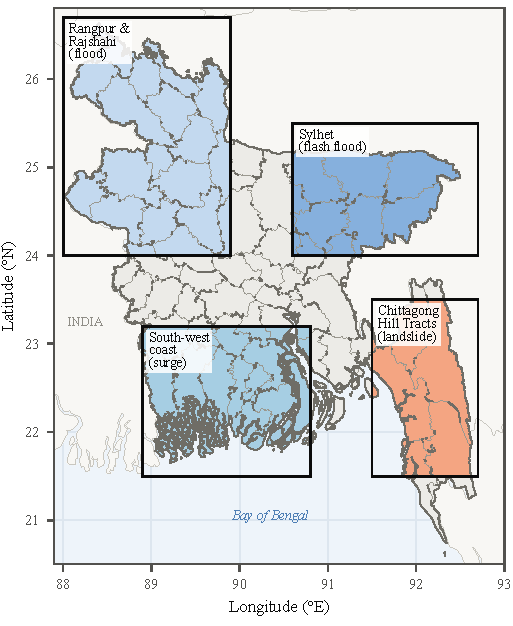
\includegraphics[width=\columnwidth]{figures/fig_study_area.pdf}
\caption{The four study regions, drawn as their configured bounding boxes over the district boundaries of geoBoundaries and tinted inside Bangladesh, blue for the three flood regions and orange for the landslide region. Neighbouring countries are from Natural Earth.}
\label{fig:study}
\end{figure}

\begin{table*}[t]
\centering
\small
\begin{tabular}{llll}
\toprule
Region & Hazard & Bounding box (W, S, E, N) & Configuration \\
\midrule
Rangpur \& Rajshahi & riverine flood & 88.0, 24.0, 89.9, 26.7 & \fileref{config.yaml} \\
Sylhet & flash flood & 90.6, 24.0, 92.7, 25.5 & \fileref{configs/sylhet.yaml} \\
South-west coast & coastal and tidal flooding & 88.9, 21.5, 90.8, 23.2 & \fileref{configs/sw\_coastal.yaml} \\
Chittagong Hill Tracts & rainfall-triggered landslide & 91.5, 21.5, 92.7, 23.5 & \fileref{configs/cht.yaml} \\
\bottomrule
\end{tabular}
\caption{Configured study regions. All use UTM zone 46N (EPSG:32646) for distance and area calculations.}
\label{tab:regions}
\end{table*}

\subsection{Data sources}

Table~\ref{tab:data} lists every dataset the pipeline ingests, and licence terms decided two of the choices. Administrative boundaries come from geoBoundaries instead of GADM because GADM forbids redistribution and therefore could not ship in the open data archive, and geoBoundaries also carries a union level, which GADM does not hold for Bangladesh. Tile providers require visible attribution, which the dashboard shows on every map, where version 1 had suppressed it. Two properties of these datasets shape what the results can say. OpenStreetMap coverage is uneven, so an area with few mapped assets shows low exposure whether or not much stands there, and the dashboard treats areas with no mapped assets as missing data and not as safe (Section~\ref{sec:aggregation}). WorldPop's constrained product carries values only where buildings were detected in imagery, so scattered rural settlement can be missed, and population exposure inherits that gap.

\begin{table*}[t]
\centering
\small
\begin{tabularx}{\textwidth}{lXll}
\toprule
Dataset & Use & Resolution & Licence \\
\midrule
OpenStreetMap & infrastructure assets (roads, bridges, schools, hospitals, shelters, embankments, cropland) & vector & ODbL 1.0 \\
SRTM 1 arc-second & elevation, slope, topographic wetness, height above drainage, flow accumulation & 30\,m & public domain \\
JRC Global Surface Water & historical water occurrence, one proxy-label vote & 30\,m & free with attribution \\
WorldPop constrained 2020 & population density for vulnerability and population exposure & 100\,m & CC BY 4.0 \\
geoBoundaries gbOpen & districts (ADM2), upazilas (ADM3), unions (ADM4) & vector & CC BY 4.0 \\
NASA COOLR & mapped landslide locations, Chittagong Hill Tracts & point & open \\
Sentinel-1 GRD (via Earth Engine) & observed flood extents for training labels and validation & 10\,m, exported at 100\,m & Copernicus open \\
\bottomrule
\end{tabularx}
\caption{Datasets ingested by the pipeline. National files (WorldPop, geoBoundaries, JRC tiles) are downloaded once into a shared cache and clipped per region.}
\label{tab:data}
\end{table*}

\section{Methods}
\label{sec:chain}

The pipeline runs as a sequence of commands, each reading the previous step's files from the region's data directory, and this section follows that chain in order. Running a region end to end is \texttt{python -m pipeline.cli -c configs/<region>.yaml run}, and each step can also be run alone. Figure~\ref{fig:chain} shows the stages and the data each one draws on.

\begin{figure*}[t]
\centering
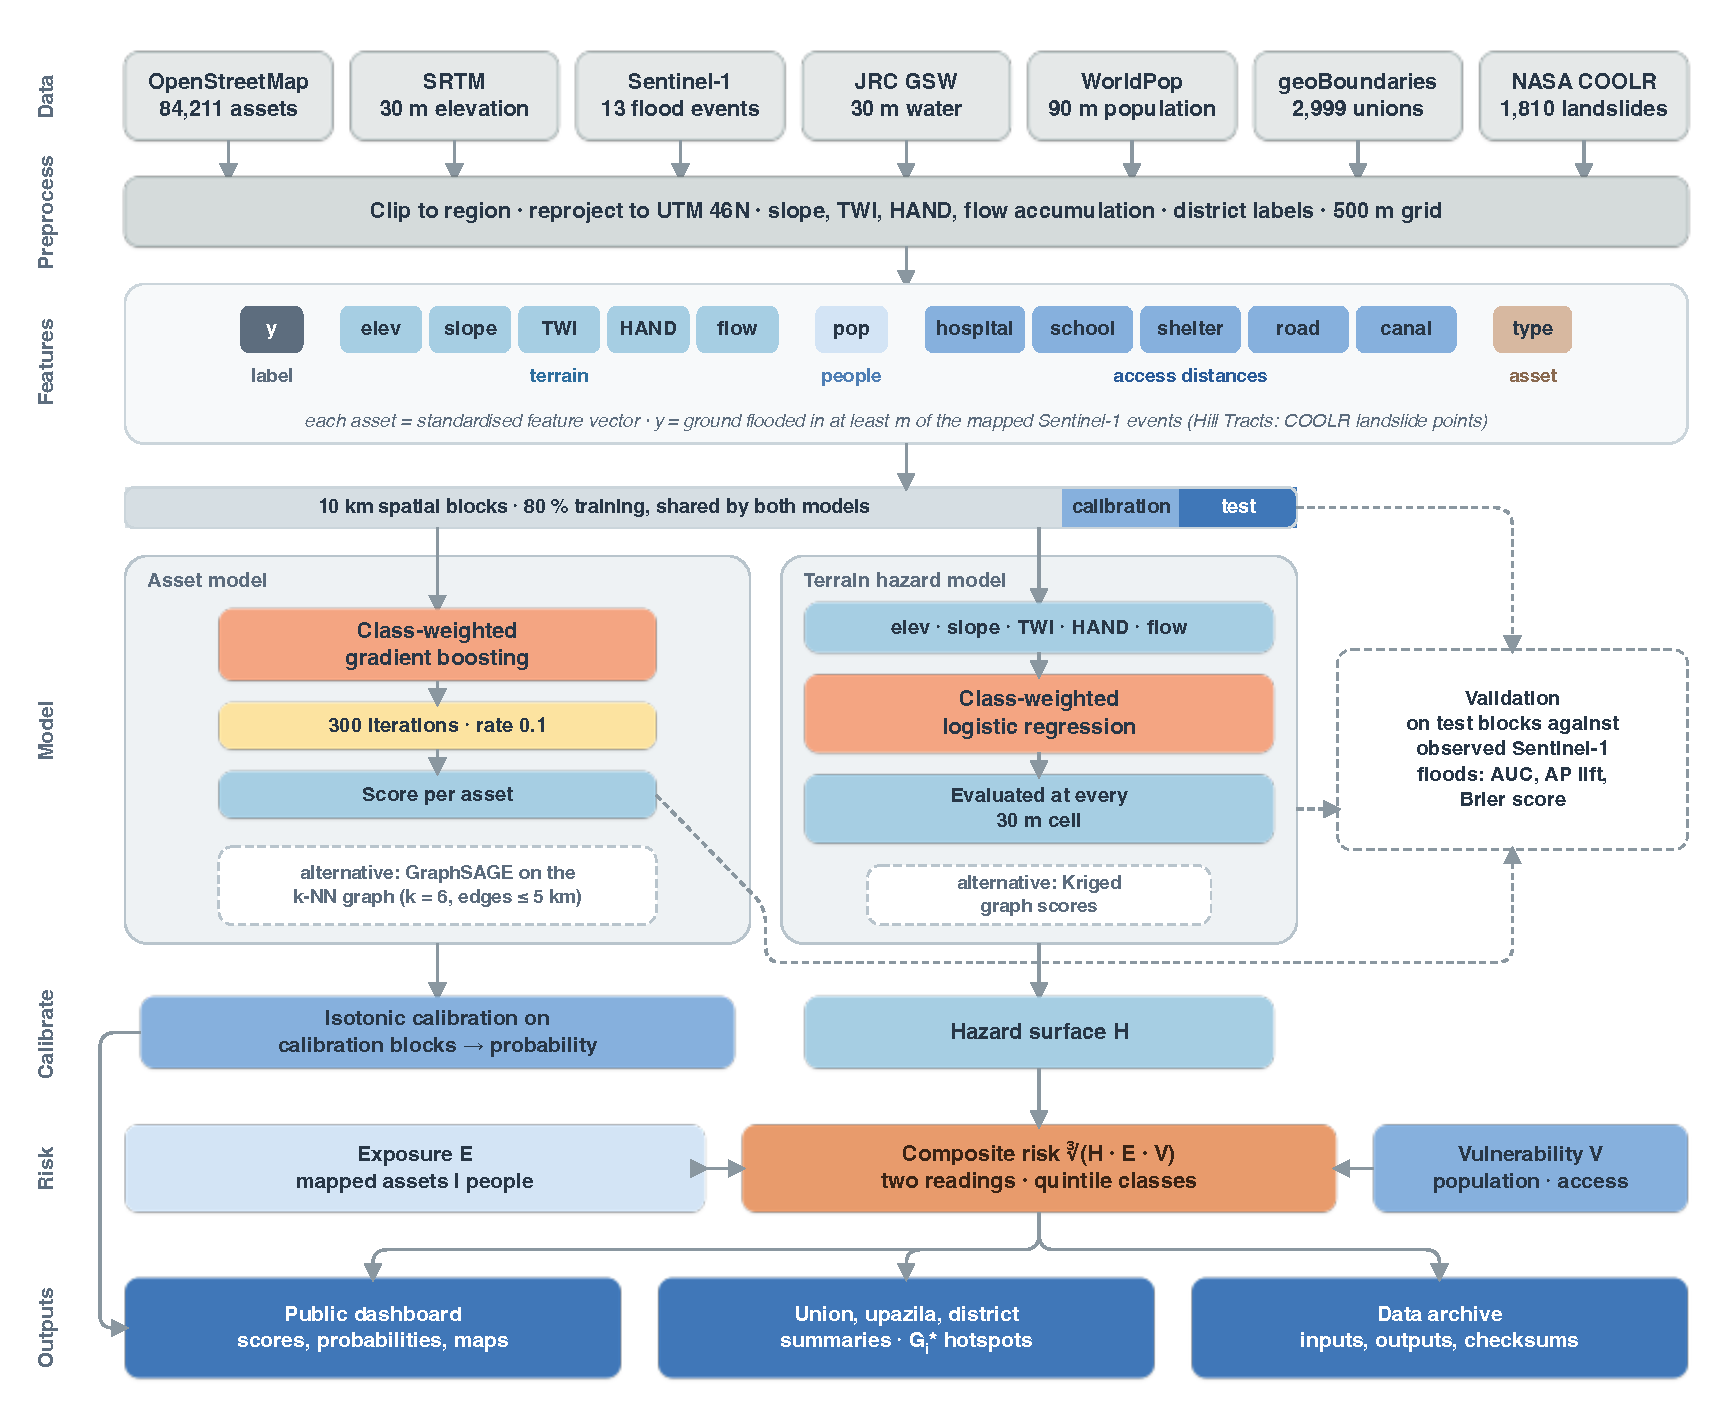
\includegraphics[width=\textwidth]{figures/fig_chain.pdf}
\caption{The processing chain, top to bottom. Source counts are totals over the three flood regions, except the landslide inventory. Each asset enters the models as a vector of terrain, population, access-distance and asset-type features, with a label from the Sentinel-1 flood frequency. The asset model is expanded, with the graph network it replaced shown as the alternative it now is. Both models train on the same spatial blocks, and dashed connectors mark what the validation scores on the test blocks. In the Chittagong Hill Tracts a landslide model fitted to the COOLR inventory takes the place of the flood labels (Section~\ref{sec:landslide}).}
\label{fig:chain}
\end{figure*}

\subsection{Infrastructure}

Assets are fetched from the Overpass API by bounding box, in tiles of 0.75$^\circ$, and clipped to the region afterwards. Version 1 queried by place name (``Rangpur Division, Bangladesh''), which returned everything in the division whether or not it lay inside the study area, and which for the hill-tracts configuration would have pulled in Chattogram city and Cox's Bazar. The tiled query also avoids the timeouts that a whole division produced, and a query refused by the Overpass server, which allows two connections per address, is retried with a growing pause, since the public mirrors tested either hung or refused connections. Three tag groups are requested, with lifeline assets covering hospitals, clinics, schools, colleges, shelters, bridges, embankments and dams, transport assets covering primary to trunk roads, railways and tagged bridges, and agricultural assets covering farmland, aquaculture, canals, ditches and marketplaces. Each feature is classified into one asset type from its tags and labelled with the district it falls in.

\subsection{Terrain derivatives}

The SRTM tiles covering the bounding box are merged, reprojected to UTM zone 46N and clipped. From the projected elevation model the pipeline derives slope, the topographic wetness index (TWI), height above nearest drainage (HAND) and D8 flow accumulation. Drainage cells for HAND are those above the 90th percentile of flow accumulation, and HAND is the elevation difference between each cell and the nearest drainage cell found by a distance transform. Flow accumulation and HAND were the slowest steps of the chain in version 1, because each was written as a per-cell Python loop, which for the Rangpur and Rajshahi elevation model meant 80 million iterations. Both are now vectorised, with the sequential part of flow accumulation compiled with numba, and produce output identical to the original implementation. The Hill Tracts elevation model now preprocesses in about two minutes, where the earlier implementation had not finished after forty minutes.

\subsection{Training labels}
\label{sec:labels}

Two label sources are supported, of which the proxy ensemble marks a pixel as flood-prone where at least two of three indicators agree, the indicators being TWI above 8, HAND below 5\,m, and JRC water occurrence above 25\,\%. This was the only source in version 1, and it is kept so the two can be compared. The proxy ensemble has a limitation that the results must carry, because TWI and HAND are also inputs to the model, so a model trained on proxy labels can succeed by relearning the threshold rule, and its validation score then measures how well it recovers that rule and not how well it anticipates flooding. The observed source replaces the ensemble with flood extents mapped from Sentinel-1 radar during past floods (Section~\ref{sec:observed}), which are independent of the terrain features. Switching between the two is a single configuration setting, and the pipeline always writes the proxy labels too, so the two can be compared.

\subsection{Features}

For each asset the pipeline samples the five terrain rasters at its representative point, samples WorldPop density, and computes the distance in metres to the nearest hospital, school, flood shelter, road and irrigation channel. Asset type enters as a categorical code, all features are standardised to zero mean and unit variance, and the label is the flood-prone status of the ground under the asset. Sampling reprojects the query coordinates into each raster's coordinate system before reading it, and the absence of that step was the central error of version 1. Longitude and latitude pairs were passed to rasters stored in UTM, every query fell outside the raster's extent, and every sampled value came back as the nodata fill of zero, which left the five terrain features constant across all assets and every label at zero. The pipeline now stops if any feature comes out constant or if the labels contain a single class.

\subsection{Asset model}
\label{sec:gnn}

The model that scores assets is a configuration setting, \texttt{asset\_model.type}, and the default is class-weighted gradient boosting over the asset features, at 300 boosting iterations with a learning rate of 0.1. That default follows from the comparison in Section~\ref{sec:benchmark}, which found ordinary tabular models matching or beating the graph network the system began with. The graph network remains available, as a two-layer GraphSAGE with 64 hidden channels and dropout of 0.3, trained with a class-weighted loss and early stopping on the calibration blocks, and so do a random forest and logistic regression. In the two riverine regions the scores shown on the map come from the same model given one more feature, the share of earlier Sentinel-1 events in which the ground flooded, trained to predict the flooding of the latest event year from the years before it and applied with the share over every event (Section~\ref{sec:temporal}). Every validation figure in this document comes from the model without that feature, because the feature is built from the same events the models are scored against.

Assets also form the nodes of a $k$-nearest-neighbour graph with $k=6$, where any pair further apart than 5\,km, measured in metres in the projected coordinate system, is left unconnected. Version 1 compared the 5\,km limit against distances in degrees, so it never removed an edge. Inverse-distance weights are stored with each edge, although the GraphSAGE mean aggregation does not use them, so every retained neighbour counts equally. Under the default model the edges carry nothing and the graph serves only to hold the features, labels and block assignment that every model shares.

Validation holds out whole spatial blocks of 10\,km instead of random nodes, because neighbouring assets share terrain, so a random split leaves every validation node next to training nodes that carry almost the same features and label, and the resulting score measures memorisation rather than skill. Blocks are assigned at random with a fixed seed to three groups, with 80\,\% for training and the remainder split evenly between calibration and test. Early stopping and the isotonic calibration of the scores use the calibration blocks only, and every metric reported in this document comes from the test blocks, which neither has seen. Isotonic regression returns the observed frequency of each level it fits, so a level holding a handful of calibration points that all flooded returns a probability of one. Each level is therefore shrunk by its Jeffreys estimate, $(k+0.5)/(n+1)$ for $k$ of $n$ points flooded, which leaves a level carrying many points almost unchanged and pulls a level carrying few back towards the middle. In Rangpur and Rajshahi the raw scores give a Brier score of \RRValBrier{} on the test blocks and the calibrated probabilities \RRValBrierCalibrated{}, against \RRValBrierBaseRate{} for always predicting the base rate, so the calibration corrects the inflated raw scores but adds little over the base rate. Flood prevalence differs from one set of blocks to another, which limits how far a calibration carries. In Rangpur and Rajshahi \RRCalibBlockRate{}\,\% of the assets in the calibration blocks sit on flood-prone ground against \RRTestBlockRate{}\,\% in the test blocks, and a calibration fitted on the first set therefore underestimates the second (Fig.~\ref{fig:calibration}). The calibrated value is best read as an approximate probability for the region as a whole, reliable in its ranking but not in its level for any one area.

\subsection{Hazard surfaces}
\label{sec:hazard}

Two hazard surfaces are produced for every flood region, and the composite risk uses one of them according to the configuration setting \texttt{risk.hazard\_source}. The first is ordinary Kriging of the model scores at the asset locations, with a spherical variogram fitted on up to 3,000 points and a residual Kriging pass that adds back the score residuals at the nodes, and it was the only surface in version 1. How much it can say between assets depends on the spatial structure of the scores, which the fitted variogram reports. The nugget is the share of the variance that is unexplained at zero distance, and the mean Kriging variance over the full sill is the share the interpolation leaves unexplained on average. On the current runs the nugget is \RRNuggetSillRatio{} of the sill in Rangpur and Rajshahi and \SylhetNuggetSillRatio{} in Sylhet, and the mean Kriging variance is \RRKrigingSillRatio{} and \SylhetKrigingSillRatio{} of the sill respectively, so in both regions the interpolated surface smooths substantially towards the regional average. In Rangpur and Rajshahi its standard deviation across the grid is \RRKrigedGridSD{} against \RRTerrainGridSD{} for the terrain surface described next, and it varies smoothly over tens of kilometres where the terrain surface follows individual channels and levees (Fig.~\ref{fig:hazard}).

\begin{figure*}[t]
\centering
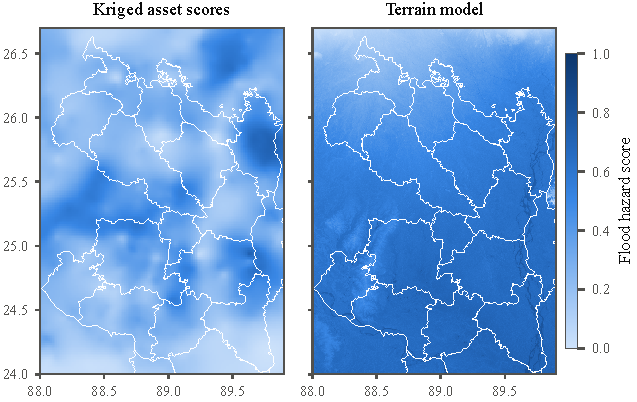
\includegraphics[width=0.8\textwidth]{figures/fig_hazard_surfaces.pdf}
\caption{The two flood hazard surfaces for Rangpur and Rajshahi, with district boundaries in white. The Kriged surface interpolates the asset model's scores between mapped assets and has a standard deviation of \RRKrigedGridSD{} across the grid. The terrain model scores each 30\,m cell from its own elevation, slope, TWI, HAND and flow accumulation, has a standard deviation of \RRTerrainGridSD{}, and reaches a cell-level AUC against observed flooding of \RRSurfaceTerrainObsAUC{}, against \RRSurfaceKrigedObsAUC{} for the Kriged surface.}
\label{fig:hazard}
\end{figure*}

The second surface is a class-weighted logistic regression from each grid cell's own terrain, using elevation, slope, TWI, HAND and flow accumulation and nothing else, because distances to hospitals or roads describe exposure and vulnerability rather than the likelihood of flooding. It is trained at the asset locations on the same labels and the same spatial blocks as the asset model, and evaluated at every grid cell, so it varies at the resolution of the elevation model rather than at the spacing of mapped infrastructure. In Rangpur and Rajshahi it reaches an AUC of \RRHazardAUC{} on held-out blocks, and it is the default. The two surfaces can also be scored directly against observed flooding over every grid cell, not only at assets, and there the terrain surface reaches an AUC of \RRSurfaceTerrainObsAUC{} against \RRSurfaceKrigedObsAUC{} for the Kriged one. Both are written to the grid so the difference between them can be inspected. Because the terrain model is trained on the observed extents, it is a flood-probability surface fitted to what the radar saw. Were it trained on the proxy labels instead, the circularity described in Section~\ref{sec:labels} would apply with full force, and it would be no more than ground the ensemble calls flood-prone, smoothed into a probability.

\subsection{Exposure}

Exposure per cell is measured twice, because ``where is infrastructure at risk'' and ``where would people be affected'' are different questions with different answers. Infrastructure exposure is the type-weighted count of mapped assets in the cell, with hospitals and schools weighted at 0.20, bridges, roads and cropland at 0.15, shelters and embankments at 0.10 and other assets at 0.05, log-scaled to the unit interval. Population exposure is WorldPop density sampled at the cell centre, log-scaled the same way. Urban municipalities lead the first measure because that is where infrastructure is concentrated, while crowded floodplain settlements can lead the second.

\subsection{Vulnerability}

Vulnerability combines population density with the distance from the cell centre to the nearest hospital, flood shelter and primary road, each normalised so that a greater distance means greater vulnerability. The configuration lists further components, a night-light proxy and an elderly-and-child ratio, that have no data source yet. Version 1 filled those with a constant of 0.5, which together with an unsampled population term made 55\,\% of the vulnerability score a constant. Components without data are now excluded and the remaining weights renormalised, and the weights actually applied are written to the output directory alongside the results. For the current runs the four applied components are population density (0.40), distance to hospital (0.27), distance to shelter (0.20) and distance to road (0.13).

\subsection{Composite risk}

Composite risk is the geometric mean of hazard, exposure and vulnerability, which keeps the multiplicative logic, in which no exposure means no risk, while staying on the unit scale of its inputs. Version 1 took the raw product and divided by its maximum, which pushed the median cell to 0.0002 against a high-risk threshold of 0.7, so no cell could ever be flagged. Two composites are written, one for each exposure measure, and both are carried through to the administrative summaries. Because the composite is bounded by its weakest factor it rarely approaches 1 even where risk is locally worst, so fixed cut-offs would place almost every cell in the lowest class. Cells are therefore also assigned relative classes 1 to 5 by quintile of the non-zero composite, the usual practice for susceptibility maps. Class 0 marks cells with no mapped exposure, which is an absence of data, not an absence of risk.

\subsection{Aggregation}
\label{sec:aggregation}

Grid results are summarised for every union, upazila and district from geoBoundaries, and each summary carries the mean and maximum of both composites, counts of exposed assets by type, and a flag stating whether the unit holds any mapped assets at all, and units without mapped assets have their risk left undefined. Version 1 filled them with zero, which the dashboard rendered as a green low-risk badge, and in Rangpur and Rajshahi that applied to \RRNUnions{} minus \RRNUnionsScored{} of the \RRNUnions{} unions. Unit names repeat across Bangladesh, so each unit also carries a label naming its parent, such as ``Abdullahpur (Gangachara)''. Hotspots are detected with the Getis--Ord $G_i^*$ statistic on $k=8$ nearest-neighbour weights, at 95\,\% confidence, over the cells that carry non-zero composite risk. Restricting the statistic to those cells keeps the weights matrix small enough to compute and avoids treating the empty majority of the grid as a sea of low values against which any occupied cell would look hot. Figure~\ref{fig:unionrisk} maps the mean composite risk of every union in the three flood regions.

\begin{figure*}[t]
\centering
\includegraphics[width=0.86\textwidth]{figures/fig_union_risk.pdf}
\caption{Mean infrastructure composite risk of each union in the three flood regions, in five relative classes by quintile of the unions scored in each region. Unions without mapped assets carry no score and are shaded as missing data, not as low risk. On the south-west coast the hazard term is close to chance against observed flooding (Section~\ref{sec:validation}), so that panel reflects mapped exposure and vulnerability more than flood hazard.}
\label{fig:unionrisk}
\end{figure*}

\section{Landslide susceptibility}
\label{sec:landslide}

The Hill Tracts region fits a susceptibility model to an observed inventory rather than assuming one. Mapped landslide locations come from NASA's Cooperative Open Online Landslide Repository (COOLR), which over the region holds \CHTLandslides{} points, all from a manual inventory of the 6~August 2023 storm mapped from PlanetScope imagery \citep{juang2019}. A class-weighted logistic regression is fitted to the five terrain derivatives at those locations against \CHTBackground{} background points, twice the number of landslides, drawn at random from the area the inventory covers and at least 500\,m from any mapped landslide. Validation holds out the same 10\,km blocks as the flood models and gives an AUC of \CHTLSAUC{} and an average precision of \CHTLSAP{} against a positive rate of \CHTLSPositiveRate{}\,\% in the test blocks. Two properties of the inventory bound what the map can claim, the first being that every point comes from one rainfall episode, so the surface describes which slopes failed in that storm, a guide to susceptibility but not a record of where landslides can occur, and the output metadata flags the inventory as single-event so that the dashboard can say so. The second is that the mapping covers only part of the region, so background points are drawn from the convex hull of the inventory, buffered by 5\,km, and not from the whole bounding box, because ground that was never mapped would otherwise enter the negative class and the model would learn the mapping footprint instead of the terrain.

The standardised coefficients are written with the model for inspection, with TWI at \CHTCoefTwi{}, HAND at \CHTCoefHand{}, flow accumulation at \CHTCoefFlowAcc{}, elevation at \CHTCoefElevation{} and slope at \CHTCoefSlope{}. The five predictors are strongly collinear, since TWI is itself computed from flow accumulation and slope, so individual coefficients describe the fit and not physical causation, the near-zero coefficient on slope should not be read as slope being unimportant, and the validation score is the number that carries the result. Version 1 applied a logistic curve to slope alone, centred on 20$^\circ$ with a scale of 5$^\circ$, that had not been fitted to any data. Where upazila boundaries were unavailable it also sliced the raster into horizontal bands, labelled each with the name of a real upazila and drew a population for it from a random number generator, and neither survives. Per-upazila statistics now come from zonal statistics over the geoBoundaries upazilas reprojected into the raster's coordinate system, and a run in which no unit overlaps the raster stops with an error instead of writing a table of zeros.

\section{Validation}
\label{sec:validation}

\subsection{Design}

Every model in the chain is scored on spatial blocks held out from training, and the same block assignment is shared by the asset model, the terrain hazard model and the landslide model within a region. Metrics are the area under the ROC curve, which measures ranking, average precision, which is more sensitive to the rare positive class, and the Brier score for calibration. Average precision is also reported as a lift over the base rate, because an average precision of 0.07 against a positive rate of 0.01 is a sevenfold improvement over chance while the same value against a rate of 0.10 is worse than chance.

\subsection{Held-out results}

Table~\ref{tab:validation} reports the asset model and the terrain hazard model for each flood region, and the landslide model for the Hill Tracts. Scores are against the observed extents on which every flood region is trained (Section~\ref{sec:observed}). The two riverine regions differ in how common flood-prone ground is under mapped assets. In Sylhet \SylhetLabelRate{}\,\% of assets sit on ground the radar saw flood and the asset model reaches an AUC of \SylhetValAUC{}. In Rangpur and Rajshahi only \RRLabelRate{}\,\% do, yet the model ranks well (AUC \RRValAUC{}) and its average precision of \RRValAP{} is a lift of \RRValAPLift{} over the base rate.

\begin{table*}[t]
\centering
\small
\begin{tabular}{lrrrrrr}
\toprule
Region & Assets & Positive rate & Asset AUC & Asset AP & Brier & Terrain AUC \\
\midrule
Rangpur \& Rajshahi & \RRAssets{} & \RRLabelRate{}\,\% & \RRValAUC{} & \RRValAP{} & \RRValBrier{} & \RRHazardAUC{} \\
Sylhet & \SylhetAssets{} & \SylhetLabelRate{}\,\% & \SylhetValAUC{} & \SylhetValAP{} & \SylhetValBrier{} & \SylhetHazardAUC{} \\
South-west coast & \CoastalAssets{} & \CoastalLabelRate{}\,\% & \CoastalValAUC{} & \CoastalValAP{} & \CoastalValBrier{} & \CoastalHazardAUC{} \\
\midrule
Chittagong Hill Tracts & \CHTLandslides{} slides & \CHTLSPositiveRate{}\,\% & \multicolumn{2}{c}{landslide AUC \CHTLSAUC{}, AP \CHTLSAP{}} & -- & -- \\
\bottomrule
\end{tabular}
\caption{Validation on held-out 10\,km test blocks, for the single block assignment behind the published outputs. Positive rate is the share of assets on ground the radar saw flood in the required number of events. The Brier score is that of the raw class-weighted scores, and the calibrated probabilities are reported in Section~\ref{sec:gnn}. Means over repeated assignments, lower in the riverine regions and higher on the coast, are in Table~\ref{tab:benchmark}.}
\label{tab:validation}
\end{table*}

\subsection{Observed floods}
\label{sec:observed}

The independent test of the flood models is agreement with flooding that was actually observed. The pipeline maps flood extents from Sentinel-1 synthetic-aperture radar with Google Earth Engine, following the method recommended by UN-SPIDER. For each configured event the minimum VV backscatter during the flood window is compared against the median of a dry-season baseline from the same year, and a pixel is flagged as flooded where it is both dark in absolute terms (below $-16$\,dB) and at least 3\,dB darker than its baseline. Permanent water from the JRC occurrence layer, slopes above 5$^\circ$ where radar shadow mimics water, and specks smaller than eight connected pixels are removed. The masks of all events are averaged into a flood-frequency layer, and the run stops if any event has no imagery, so that an empty mask cannot pass as an absence of flooding.

Five events are configured for Rangpur and Rajshahi, four for Sylhet and four cyclone landfalls for the south-west coast (Table~\ref{tab:events}). Each window was set from ReliefWeb situation reports and the source is recorded against the event in the region configuration, so a reader can check the dates and a later run can add events the same way. Figure~\ref{fig:frequency} shows the resulting flood-frequency layers.

The masks were also checked against an independent map of the same floods. The Global Flood Database maps flood events from MODIS optical imagery at 250\,m \citep{tellman2021}, and two of its events coincide with events mapped here, the August 2017 flood in Rangpur and Rajshahi and the April 2017 haor flood in Sylhet. The comparison runs on the database's grid, inside Bangladesh and over cells that MODIS saw clear at least once and that are not permanent water, and a cell counts as flooded by radar where at least half of it flooded. The two maps agree on \RRXcAgree{}\,\% of \RRXcCells{} cells in Rangpur and Rajshahi and \SylhetXcAgree{}\,\% of \SylhetXcCells{} in Sylhet, a figure dominated by dry ground, while on flooded ground the agreement is moderate, with a critical success index of \RRXcCSI{} and \SylhetXcCSI{} and a kappa of \RRXcKappa{} and \SylhetXcKappa{}. The disagreement runs in opposite directions. In Rangpur and Rajshahi the radar marks \RRXcSOneShare{}\,\% of the cells as flooded against \RRXcGfdShare{}\,\% for MODIS, a false alarm ratio of \RRXcFAR{}, which is consistent with flooded patches smaller than a 250\,m pixel and with flooding hidden from an optical sensor by monsoon cloud. In the Sylhet haor the radar marks \SylhetXcSOneShare{}\,\% against \SylhetXcGfdShare{}\,\% and detects \SylhetXcPOD{} of the flooding MODIS saw, which is consistent with the known difficulty of radar where water stands under vegetation \citep{amitrano2024}, as it did under the unharvested rice of April 2017. Neither explanation was tested, and neither map is ground truth, so the comparison bounds what the labels can claim rather than measuring their error.

\begin{figure*}[t]
\centering
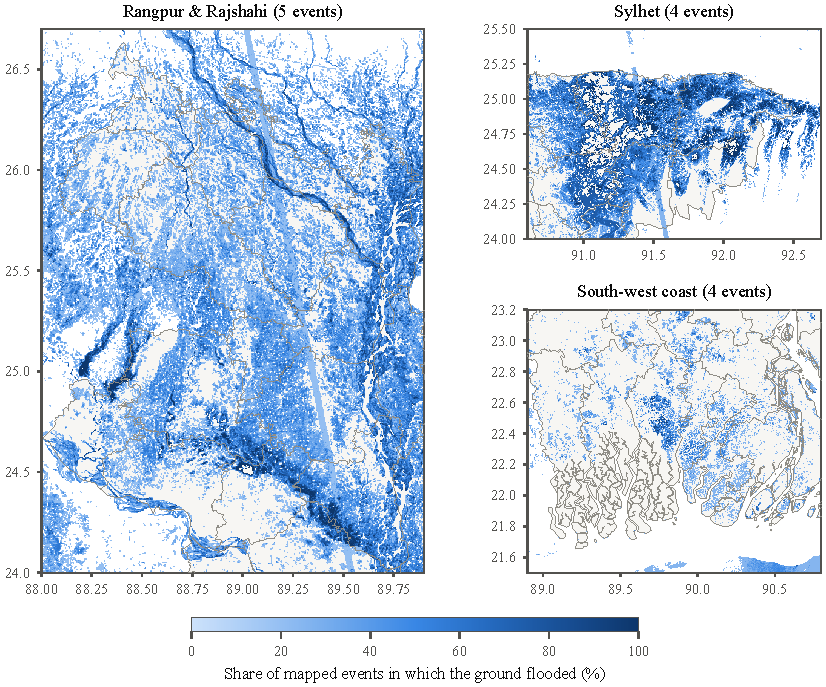
\includegraphics[width=0.86\textwidth]{figures/fig_flood_frequency.pdf}
\caption{Share of the mapped Sentinel-1 events in which each 100\,m cell was flooded, for the three flood regions. Cells never seen flooded are left blank, and the removal of permanent water leaves the main river channels empty. Straight-edged bands follow the edges of radar swaths.}
\label{fig:frequency}
\end{figure*}

\begin{table*}[t]
\centering
\small
\begin{tabularx}{\textwidth}{llX}
\toprule
Region & Window & Basis \\
\midrule
Rangpur \& Rajshahi & 12--26 Aug 2017 & second monsoon flood from 12 August; Dinajpur, Kurigram, Lalmonirhat and Rangpur among the worst affected \\
 & 12--26 Jul 2019 & rain from 9 July, Brahmaputra--Jamuna rising to 18 July, Kurigram more than 1\,m above danger level \\
 & 11--31 Jul 2020 & second phase from 9--10 July, peak about 18 July, 27 basin gauges above danger into late July \\
 & 28 Jun--16 Jul 2024 & northern floods from mid-June, Brahmaputra above danger at Nunkhawa, Hatia and Chilmari in early July \\
 & 27 Sep--12 Oct 2024 & Teesta flooding of Lalmonirhat, Nilphamari, Kurigram and Rangpur from late September \\
\midrule
Sylhet & 30 Mar--20 Apr 2017 & haor flooding from 28 March, striking Sunamganj on 1 April \\
 & 15--26 Jun 2022 & heavy rain from 15 June, situation worst from 17 June \\
 & 16--28 Jun 2024 & 2.25 million affected in Sylhet, Sunamganj and Moulvibazar by 22 June \\
 & 18--30 Aug 2024 & eastern floods from 20 August, including Moulvibazar and Habiganj \\
\midrule
South-west coast & 20--31 May 2020 & Cyclone Amphan, landfall 20 May \\
 & 25 May--4 Jun 2021 & Cyclone Yaas, landfall 26 May \\
 & 23 Oct--2 Nov 2022 & Cyclone Sitrang, landfall 24--25 October \\
 & 26 May--5 Jun 2024 & Cyclone Remal, landfall 26--27 May \\
\bottomrule
\end{tabularx}
\caption{Flood events mapped from Sentinel-1. Windows bracket the flood peak; the baseline for each is the February--March dry season of the same year (mid-January to March for the pre-monsoon haor event). Sources are ReliefWeb situation reports, cited in the configuration files.}
\label{tab:events}
\end{table*}

The validation step then answers three questions separately. Whether model scores rank assets that flooded above those that did not is measured on the held-out blocks. Whether the hazard surface agrees with observed flooding across the whole grid, and not only where assets happen to be, is measured by AUC and Spearman correlation over all cells. And how closely the proxy labels match observed flooding is measured with the categorical scores used in flood mapping, the probability of detection, false alarm ratio and critical success index, which quantifies what the proxy-trained models were learning.

\label{sec:labelresult}
The comparison of the proxy labels with observed flooding shows what they do and do not capture. In Rangpur and Rajshahi the terrain ensemble captures \RRProxyPOD{} of the ground that flooded in at least \RRMinEvents{} of the five events (probability of detection), with a false alarm ratio of \RRProxyFAR{} and a critical success index of \RRProxyCSI{}. It marks \RRProxyShare{}\,\% of the region as flood-prone where the radar saw \RRObservedShare{}\,\% flood that often, so as a map it covers much less ground than the flooding that occurred. A model trained on it still ranks above chance, because terrain wetness orders ground by flood-proneness even where the thresholded labels miss the flood itself, but it pays for the labels it was given. Retrained on the proxy labels and scored on the same held-out blocks against the same observed definition, over \RRBenchSeeds{} block assignments, it reaches an AUC of \RRLabelProxyAUC{} in Rangpur and Rajshahi against \RRLabelObsAUC{} for observed labels, a gap of \RRLabelGap{} ($p\RRLabelGapP{}$) with the observed labels ahead on \RRLabelAhead{} of \RRBenchSeeds{} assignments. Sylhet gives \SylhetLabelProxyAUC{} against \SylhetLabelObsAUC{}, ahead on \SylhetLabelAhead{}, and the coast \CoastalLabelProxyAUC{} against \CoastalLabelObsAUC{}, ahead on \CoastalLabelAhead{} (Fig.~\ref{fig:roc}). This comparison favours the observed labels, since the model trained on them is scored against the definition it learned while the proxy-trained model is scored against one it never saw, and Section~\ref{sec:temporal} therefore repeats it against later floods that neither label source was trained on. The model of version 1 is not among these, since its labels were all zero (Section~\ref{sec:corrections}) and it had nothing to learn from.

The models are consequently trained on the observed extents. In the riverine regions a pixel counts as flood-prone where it flooded in at least two of the mapped events, five in Rangpur and Rajshahi and four in Sylhet, while on the coast one of the four cyclone windows is enough, because surge flooding drains within days and the six-to-twelve-day Sentinel-1 revisit leaves too few pixels flooded twice to train on. Validation on held-out blocks against the same definition gives an AUC of \RRValAUC{} and a precision lift of \RRValAPLift{} in Rangpur and Rajshahi, \SylhetValAUC{} and \SylhetValAPLift{} in Sylhet, and \CoastalValAUC{} and \CoastalValAPLift{} on the coast. The same model trained on proxy labels instead trails it by between \CoastalLabelGap{} and \RRLabelGap{} in AUC, averaged over the \RRBenchSeeds{} block assignments (Fig.~\ref{fig:roc}).

\begin{figure*}[t]
\centering
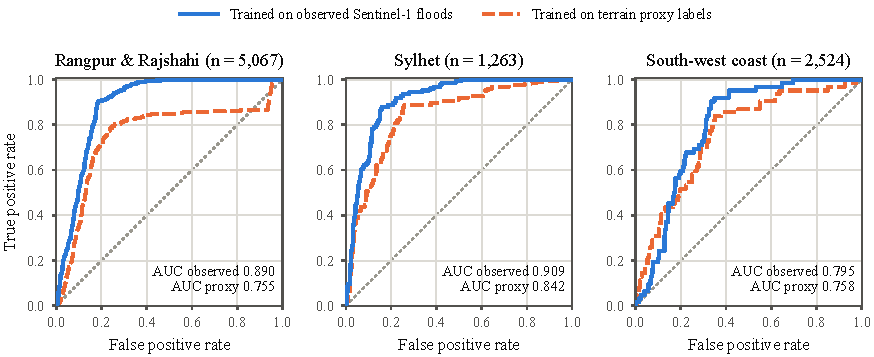
\includegraphics[width=\textwidth]{figures/fig_roc.pdf}
\caption{ROC curves on the held-out test blocks of each flood region, scored against the observed definition of flood-prone ground. Both curves come from the default gradient-boosted model on one block assignment, sharing features and blocks and differing only in their training labels. The dotted diagonal is a random ranking, and $n$ is the number of assets in the test blocks.}
\label{fig:roc}
\end{figure*}

\begin{figure*}[t]
\centering
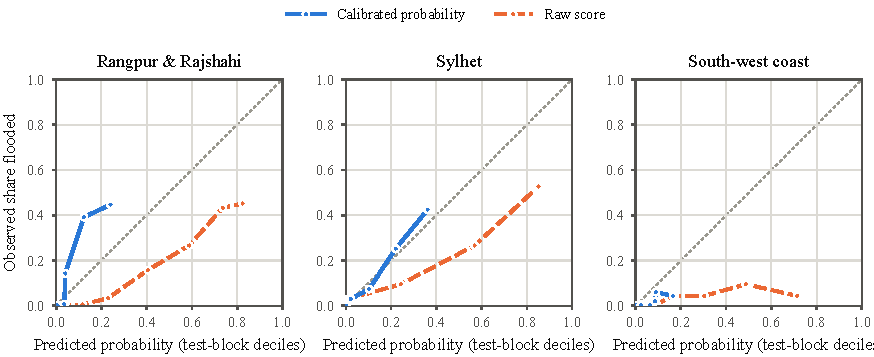
\includegraphics[width=\textwidth]{figures/fig_calibration.pdf}
\caption{Reliability of the flood model on the test blocks, with assets grouped into deciles of each prediction. The raw class-weighted score overstates the likelihood of flooding. The isotonic calibration corrects most of that overstatement but was fitted on other blocks, and where the test blocks hold more flood-prone ground than the calibration blocks, as in Rangpur and Rajshahi (\RRTestBlockRate{}\,\% against \RRCalibBlockRate{}\,\%), its top deciles lie above the diagonal and understate the flooding observed.}
\label{fig:calibration}
\end{figure*}

The south-west coast behaves differently from the two riverine regions. The asset model still ranks the ground that flooded above the ground that did not, with an AUC of \CoastalValAUC{} and a precision lift of \CoastalValAPLift{}, but across the whole grid both hazard surfaces are close to chance, the terrain surface scoring \CoastalSurfaceTerrainObsAUC{} and the Kriged one \CoastalSurfaceKrigedObsAUC{}. Surge flooding is governed by polder embankments, tidal channels and where a storm makes landfall, none of which the elevation-derived predictors describe, so the coastal hazard layer should not be read as a map of surge exposure, and a coastal model would need embankment and tide data that the pipeline does not yet ingest. Two caveats apply to the radar extents themselves. Inundated paddy is open water to a radar and is counted as flooding, which is one reason the two-event threshold is preferred where the data allow it. And the minimum-backscatter composite over a window of two weeks records the largest extent reached at any pass in the window, not the extent on any one day.

\subsection{Transfer to later floods}
\label{sec:temporal}

The held-out blocks separate training from testing in space but not in time, since the labels and the reference extents come from the same events, while a map is meant to anticipate a flood that has not yet happened. Each flood model is therefore also trained on labels from the events up to 2022, which are 2017, 2019 and 2020 in Rangpur and Rajshahi, 2017 and 2022 in Sylhet and the three cyclones from 2020 to 2022 on the coast, and scored on the held-out blocks against the extents of the 2024 events. The training labels keep each region's rule, capped by the number of earlier events, so ground counts as flood-prone where it flooded in at least two of three events in Rangpur and Rajshahi, in both events in Sylhet and in at least one cyclone on the coast, and it counts as flooded in 2024 where any 2024 event reached it. Three references are scored on the same assets over the same \RRTempSeeds{} block assignments. The first is the share of the earlier events in which the ground flooded, which is the map a planner would hold from the radar record alone, the second is the same model trained on labels that include the 2024 events, which is the spatial-only design of Section~\ref{sec:observed}, and the third is the same model trained on the terrain-threshold labels of Section~\ref{sec:labels}, which draw on no flood event.

\begin{table*}[t]
\centering
\small
\begin{tabular}{lcccc}
\toprule
Region & Model to 2022 & All events & Past flooding & Terrain labels \\
\midrule
Rangpur \& Rajshahi & \RRTempAUC{} $\pm$ \RRTempSD{} & \RRTempAllAUC{} & \RRTempPastAUC{} $\pm$ \RRTempPastSD{} & \RRTempProxyAUC{} $\pm$ \RRTempProxySD{} \\
Sylhet & \SylhetTempAUC{} $\pm$ \SylhetTempSD{} & \SylhetTempAllAUC{} & \SylhetTempPastAUC{} $\pm$ \SylhetTempPastSD{} & \SylhetTempProxyAUC{} $\pm$ \SylhetTempProxySD{} \\
South-west coast & \CoastalTempAUC{} $\pm$ \CoastalTempSD{} & \CoastalTempAllAUC{} & \CoastalTempPastAUC{} $\pm$ \CoastalTempPastSD{} & \CoastalTempProxyAUC{} $\pm$ \CoastalTempProxySD{} \\
\bottomrule
\end{tabular}
\caption{AUC against the 2024 flood extents on held-out 10\,km test blocks, as mean $\pm$ standard deviation over \RRTempSeeds{} block assignments. The model to 2022 is trained only on the earlier events, the all-events model on labels that include 2024, past flooding is the share of the earlier events in which the ground flooded, and the terrain-label model is the same model trained on the terrain-threshold labels. The 2024 events reached \RRTempTestRate{}\,\%, \SylhetTempTestRate{}\,\% and \CoastalTempTestRate{}\,\% of assets in the three regions.}
\label{tab:temporal}
\end{table*}

Trained only on the earlier floods, the model ranks the ground the 2024 floods reached at an AUC of \RRTempAUC{} in Rangpur and Rajshahi, \SylhetTempAUC{} in Sylhet and \CoastalTempAUC{} on the coast (Table~\ref{tab:temporal}). In Rangpur and Rajshahi leaving the 2024 events out of training costs nothing measurable ($p\RRTempMinusAllP{}$), while in Sylhet and on the coast it costs \SylhetTempAllGap{} and \CoastalTempAllGap{} in AUC, which is the price of anticipating a flood the model has not seen. The comparison with past flooding is the more instructive one. In both riverine regions the radar record of the earlier floods ranks the 2024 flooding better than the model does, at \RRTempPastAUC{} against \RRTempAUC{} in Rangpur and Rajshahi, where the model is ahead on \RRTempAheadPast{} of \RRTempSeeds{} assignments, and \SylhetTempPastAUC{} against \SylhetTempAUC{} in Sylhet, where it is ahead on \SylhetTempAheadPast{}. On the coast the order reverses, with the model ahead at \CoastalTempAUC{} against \CoastalTempPastAUC{} on \CoastalTempAheadPast{} of \CoastalTempSeeds{} assignments.

The likely reading is that riverine flooding returns to much the same ground from one monsoon to the next, so that the footprint of several observed floods is already a strong guide to the next one, whereas each cyclone surge floods the stretch of coast where it makes landfall. The 2024 floods bear this out, since \RRPastFeatUnseenPos{}\,\% of the flooded assets in Rangpur and Rajshahi and \SylhetPastFeatUnseenPos{}\,\% in Sylhet stood on ground no earlier event had reached, against \CoastalPastFeatUnseenPos{}\,\% on the coast.

The record of earlier flooding can also be given to the model as a feature, provided it comes from floods before the ones the model learns to predict, since a feature drawn from the training events would let the model copy its own labels. The model is therefore trained to predict the flooding of the last event year up to 2022 from its usual features and the share of the events before that year in which the ground flooded, and it is scored on the held-out blocks against the 2024 floods with the share taken over all the events up to 2022. In the riverine regions the combination outperforms both of its parts. It reaches \RRPastFeatAUC{} in Rangpur and Rajshahi and \SylhetPastFeatAUC{} in Sylhet, against \RRPastFeatOnlyAUC{} and \SylhetPastFeatOnlyAUC{} for past flooding alone, ahead on \RRPastFeatOverPastAhead{} and \SylhetPastFeatOverPastAhead{} of \RRTempSeeds{} assignments ($p\RRPastFeatOverPastP{}$ and $p\SylhetPastFeatOverPastP{}$), and against \RRPastFeatWithoutAUC{} and \SylhetPastFeatWithoutAUC{} for the same model trained on the same target without the feature. The terrain and access features therefore add to the flood record rather than repeat it, and they do so on the ground no earlier flood reached, where past flooding gives every asset the same score of zero. That ground holds \RRPastFeatUnseenShare{}\,\% of the test assets in Rangpur and Rajshahi and \SylhetPastFeatUnseenShare{}\,\% in Sylhet, and on it the combined model ranks the 2024 flooding at \RRPastFeatUnseenAUC{} and \SylhetPastFeatUnseenAUC{}, where past flooding alone can do no better than chance. On the coast the design is weaker, because it leaves a single cyclone to train on, and the combination at \CoastalPastFeatAUC{} cannot be told apart from past flooding alone at \CoastalPastFeatOnlyAUC{} ($p\CoastalPastFeatOverPastP{}$), both well below the \CoastalTempAUC{} of the model trained on all three earlier cyclones. The riverine maps published with this study use the feature, trained in this way and applied with the share taken over every mapped event (Section~\ref{sec:gnn}), while every other validation figure comes from the model without it.

The 2024 floods also give the label comparison of Section~\ref{sec:labelresult} a test that favours neither label source. There the model trained on observed extents is scored against the definition it learned and the model trained on terrain labels against one it never saw, whereas neither has seen the 2024 floods. The observed labels still lead, at \RRTempAUC{} against \RRTempProxyAUC{} in Rangpur and Rajshahi, \SylhetTempAUC{} against \SylhetTempProxyAUC{} in Sylhet and \CoastalTempAUC{} against \CoastalTempProxyAUC{} on the coast, ahead on \RRTempProxyAhead{}, \SylhetTempProxyAhead{} and \CoastalTempProxyAhead{} of \RRTempSeeds{} assignments ($p\RRTempProxyGapP{}$, $p\SylhetTempProxyGapP{}$ and $p\CoastalTempProxyGapP{}$). The gap of \RRTempProxyGap{} in Rangpur and Rajshahi matches the \RRLabelGap{} of the spatial comparison and the coastal gap of \CoastalTempProxyGap{} stays close to its \CoastalLabelGap{}, while in Sylhet the gap falls from \SylhetLabelGap{} to \SylhetTempProxyGap{}, so part of the Sylhet advantage in the spatial comparison came from scoring against the definition the observed model was trained on rather than from the labels themselves.


\subsection{Model comparison}
\label{sec:benchmark}

A score means little without something to compare it against, so the graph network the system was built around is set against ordinary models that see the same standardised features at the same assets and are trained and scored on the same blocks. The comparison covers class-weighted logistic regression, a random forest and gradient boosting, with the topographic wetness index alone as a model-free reference. Every model is refitted on \RRBenchSeeds{} block assignments drawn with different seeds, because one assignment gives a single number with no sense of how much of any gap is noise, and Table~\ref{tab:benchmark} reports the mean and standard deviation across those assignments (Fig.~\ref{fig:benchmark}).

The graph structure does not pay for itself. In every region the graph network trails the best of the ordinary models. In Rangpur and Rajshahi it averages \RRBenchGraphAUC{} against \RRBenchForestAUC{} for the random forest and \RRBenchBoostingAUC{} for gradient boosting, trailing the best by \RRBenchGap{} in AUC ($p\RRBenchDiffP{}$, paired across assignments) and ahead on \RRBenchAhead{} of \RRBenchSeeds{} assignments. In Sylhet it averages \SylhetBenchGraphAUC{} against \SylhetBenchForestAUC{} for the random forest, behind by \SylhetBenchGap{} ($p\SylhetBenchDiffP{}$) and ahead on \SylhetBenchAhead{} of \SylhetBenchSeeds{}. On the south-west coast it trails gradient boosting by \CoastalBenchGap{}, which at $p\CoastalBenchDiffP{}$ cannot be told apart from no difference, and it is ahead on \CoastalBenchAhead{} of \CoastalBenchSeeds{} assignments. Gradient boosting and the random forest differ by less than 0.01 in mean AUC in every region and cannot be told apart on paired tests. The wetness index alone ranks little better than chance everywhere, at \RRBenchTwiAUC{} in Rangpur and Rajshahi, \SylhetBenchTwiAUC{} in Sylhet and \CoastalBenchTwiAUC{} on the coast, so the wetness index carries little of the signal on its own, and an ordinary tabular model extracts it from the full set of features at least as well as the graph does. Gradient boosting is consequently the default model of the system, and the results reported elsewhere in this document come from it, with the graph network kept as a configuration option rather than as the method. A single default is kept for every region, since choosing a different model for each would fit the model to the split as well as to the region.

The spread across assignments also governs how the other numbers in this document should be read. The default model's AUC varies by \RRBenchBoostingSD{} in Rangpur and Rajshahi, \SylhetBenchBoostingSD{} in Sylhet and \CoastalBenchBoostingSD{} on the coast from one assignment to the next. Several differences this document reports are of that size, so each is quoted with the assignments behind it, and every figure that comes from the single assignment behind the published outputs, including those in Table~\ref{tab:validation}, should be read as one draw from a distribution of that width rather than as a fixed property of the system.

\begin{table*}[t]
\centering
\small
\begin{tabular}{lccc}
\toprule
Model & Rangpur \& Rajshahi & Sylhet & South-west coast \\
\midrule
Graph model (GraphSAGE) & \RRBenchGraphAUC{} $\pm$ \RRBenchGraphSD{} & \SylhetBenchGraphAUC{} $\pm$ \SylhetBenchGraphSD{} & \CoastalBenchGraphAUC{} $\pm$ \CoastalBenchGraphSD{} \\
Gradient boosting & \RRBenchBoostingAUC{} $\pm$ \RRBenchBoostingSD{} & \SylhetBenchBoostingAUC{} $\pm$ \SylhetBenchBoostingSD{} & \CoastalBenchBoostingAUC{} $\pm$ \CoastalBenchBoostingSD{} \\
Random forest & \RRBenchForestAUC{} $\pm$ \RRBenchForestSD{} & \SylhetBenchForestAUC{} $\pm$ \SylhetBenchForestSD{} & \CoastalBenchForestAUC{} $\pm$ \CoastalBenchForestSD{} \\
Logistic regression & \RRBenchLogisticAUC{} $\pm$ \RRBenchLogisticSD{} & \SylhetBenchLogisticAUC{} $\pm$ \SylhetBenchLogisticSD{} & \CoastalBenchLogisticAUC{} $\pm$ \CoastalBenchLogisticSD{} \\
Wetness index alone & \RRBenchTwiAUC{} $\pm$ \RRBenchTwiSD{} & \SylhetBenchTwiAUC{} $\pm$ \SylhetBenchTwiSD{} & \CoastalBenchTwiAUC{} $\pm$ \CoastalBenchTwiSD{} \\
\midrule
Graph minus best baseline & \RRBenchDiff{} & \SylhetBenchDiff{} & \CoastalBenchDiff{} \\
\bottomrule
\end{tabular}
\caption{AUC on held-out test blocks, as mean $\pm$ standard deviation over \RRBenchSeeds{} block assignments. Every model sees the same features at the same assets and the same blocks, so the only difference is the model. The last row is the paired difference between the graph network and whichever other model scores best in that region. Gradient boosting is the system's default.}
\label{tab:benchmark}
\end{table*}

\begin{figure*}[t]
\centering
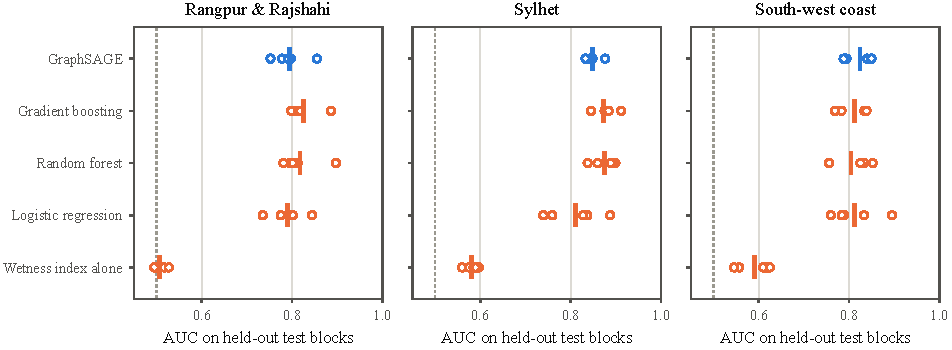
\includegraphics[width=\textwidth]{figures/fig_benchmark.pdf}
\caption{AUC of each model on the held-out test blocks, one circle per block assignment and a vertical bar at the mean. The graph network is in blue, the other models in orange, and the dotted line marks a random ranking. The graph network sits inside the range of the ordinary models in every region.}
\label{fig:benchmark}
\end{figure*}

\subsection{What the model relies on}
\label{sec:importance}

Shuffling each feature across the test assets and recording the loss in AUC, over the same \RRBenchSeeds{} block assignments, shows what the default model uses (Fig.~\ref{fig:importance}). Elevation carries almost all of the terrain signal, costing \RRImpElevation{} in AUC when shuffled in Rangpur and Rajshahi, \SylhetImpElevation{} in Sylhet and \CoastalImpElevation{} on the coast, while the wetness index, height above drainage, slope and flow accumulation cost no more than \RRImpOtherTerrainMax{}, \SylhetImpOtherTerrainMax{} and \CoastalImpOtherTerrainMax{} each. Because shuffling one of several correlated features understates each of them, the five terrain features were also shuffled together, and they cost \RRImpTerrain{}, \SylhetImpTerrain{} and \CoastalImpTerrain{}, little more than elevation alone, so the derived terrain indices add almost nothing once elevation is known. The five access distances, shuffled together, are the second group at \RRImpAccess{}, \SylhetImpAccess{} and \CoastalImpAccess{}, ahead of population density and asset type. These distances describe how far an asset lies from services rather than any property of flooding, and they most likely stand in for where roads and settlements sit on the floodplain, which would give the tabular model much of the spatial information the graph was meant to supply, although that reading was not tested directly. The terrain hazard surface of Section~\ref{sec:hazard} leaves them out, since it scores ground rather than assets.

\begin{figure*}[t]
\centering
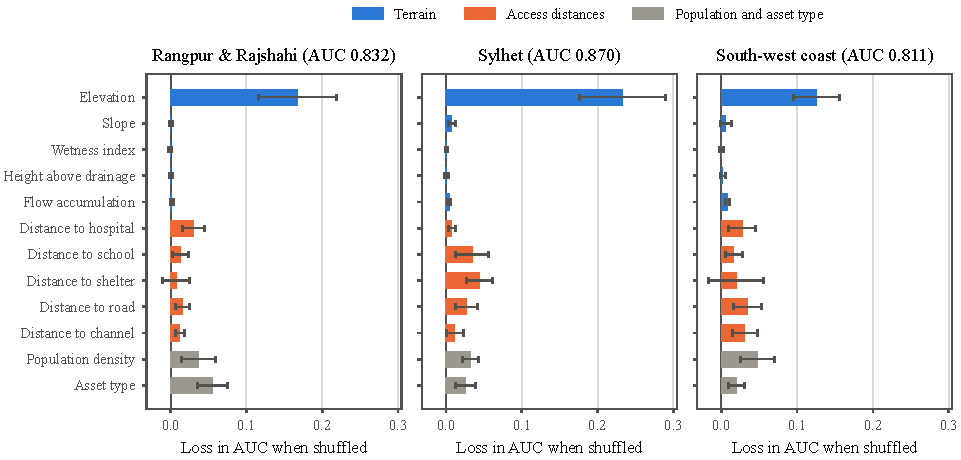
\includegraphics[width=\textwidth]{figures/fig_importance.pdf}
\caption{Loss in AUC on the held-out test blocks when each feature is shuffled across the test assets, as mean and standard deviation over \RRBenchSeeds{} block assignments, for the default gradient-boosted model. The AUC in each title is the mean before shuffling.}
\label{fig:importance}
\end{figure*}

\subsection{Weight sensitivity}
\label{sec:sensitivity}

The composite risk rests on weights that were chosen rather than measured, so the ranking it produces is recomputed under other defensible choices and compared with the published one by Spearman correlation and by the share of the top decile of cells that stays in the top decile. Weighting every asset type equally leaves the ordering almost unchanged, at $\rho=\RRSensEqualTypesRho{}$ in Rangpur and Rajshahi and $\rho=\CoastalSensEqualTypesRho{}$ on the coast, and so does weighting the vulnerability components equally. Doubling the exposure exponent in the geometric mean gives $\rho=\RRSensExposureDoubleRho{}$ while retaining \RRSensExposureDoubleTop{} of the top decile. Multiplying every chosen weight by a random factor between 0.5 and 1.5, over \RRSensDraws{} draws, gives a mean $\rho$ of \RRSensRandomRho{} in Rangpur and Rajshahi, \SylhetSensRandomRho{} in Sylhet and \CoastalSensRandomRho{} on the coast, with \RRSensRandomTop{} of the top decile retained.

Only one choice matters, reducing vulnerability to population density alone, which discards the distances to hospitals, shelters and roads and drops the correlation to \RRSensPopOnlyRho{} in Rangpur and Rajshahi and \CoastalSensPopOnlyRho{} on the coast, so the access distances rather than population drive the vulnerability term. The ordering of cells is therefore not an artefact of the particular weights, while the boundary of the top class is soft enough that a cell just inside it and a cell just outside should be treated alike.

\section{Dashboard}

The dashboard is a Streamlit application open to anyone, with a region selector once more than one region has results. Every number it shows is read from a pipeline output file, and when a file is missing the page says so instead of substituting a placeholder. A test in the repository fails if any dashboard module reintroduces mock data, an authentication gate or random values. A flood region shows four tabs, of which the risk map draws asset markers sized by score, the composite-risk heatmap, union boundaries coloured by mean risk with unscored units in grey, hotspots, and optional terrain and hazard overlays that are pre-rendered in WGS84 because a projected raster placed by latitude and longitude corners would land in the wrong place. Popups show the asset's score and the hazard, exposure and vulnerability of its cell, taken from the grid and not derived from the score. The rankings tab lists the highest-scoring assets, the union summaries with both exposure readings, and downloads. The preparedness tab lists the official warning sources and the flood shelters mapped in OpenStreetMap, stating that capacity and opening status are not known. The about tab explains the method in plain language, names every data source with its licence, and lists the known limitations. A landslide region shows its susceptibility surface, the fitted coefficients in plain words, and the per-upazila table, with the single-event caveat placed above the map.

The sidebar reports provenance: when the region was processed, the number of assets, the label positive rate, the validation AUC and Brier score, the Kriging variance and its ratio to the sill, and, where available, the observed-flood validation and the landslide model's inventory size and AUC. Version 1 of the dashboard sat behind a login whose credentials were printed on the login page, and displayed volunteer responders with telephone numbers, cash-transfer programmes with disbursement figures, shelters marked open or at capacity, monthly risk curves for 2024 to 2026 and a pipeline status panel reading ``BWDB gauges 43/45 live''. None of it was connected to any data source, and all of it has been removed.

\section{Deployment}

The application runs as a systemd service on the same host as \url{fermium.systems}, behind nginx. Streamlit binds to the loopback address only, with cross-site request forgery protection enabled, uploads capped at 1\,MB and error details hidden from visitors. Nginx terminates TLS, adds security headers including a content security policy limited to the tile and font origins the page uses, and applies per-address limits of ten requests per second with a burst of thirty and twelve concurrent connections, because each open browser tab holds a websocket and a copy of the region's data in the server's memory. The service unit caps memory at 4\,GB, restricts the process to reading its own directory, and restarts on failure. Display caches are rebuilt with \texttt{python preprocess\_cache.py -c <config>} after every pipeline run, which converts the GeoJSON outputs to GeoParquet and simplifies administrative geometry to a 50\,m tolerance, reducing the union layer from 36\,MB to 2\,MB.

\section{Limitations}
\label{sec:limitations}

The limitations below are stated on the dashboard as well as here, and the first governs how every validation figure should be read. The flood labels and the flood extents the models are scored against come from the same Sentinel-1 events, so the held-out blocks separate training from testing in space but not in time. Scored against the 2024 floods after training on earlier ones, the models lose up to \CoastalTempAllGap{} in AUC, and in the two riverine regions the record of earlier flooding predicts the next flood better than the model does unless the model is given that record as a feature (Section~\ref{sec:temporal}). The riverine maps published with this document include the feature, although every validation figure outside Section~\ref{sec:temporal} comes from the model without it. Inundated paddy also appears as open water to radar and is counted as flooding. Composite risk is defined only where OpenStreetMap has mapped assets, which in Rangpur and Rajshahi is \RRMappedCellShare{}\,\% of grid cells, and units without mapped assets are reported as missing rather than as low risk. Sparse mapping therefore reads as low exposure and not as low risk, and the infrastructure composite rises with asset density and is led by urban municipalities, which is the intended reading for infrastructure at risk and not a measure of risk to people, for which the population composite exists.

Vulnerability uses population density and three access distances, so income, housing quality and age structure are not represented, and WorldPop's constrained product misses settlement outside detected buildings. No model tried here does measurably better than a gradient-boosted tree on the same features, and the graph network the system began with is worse in every region, measurably so in the two riverine ones (Section~\ref{sec:benchmark}). The tree is therefore the default, and its advantage rests on the features rather than on anything the architecture contributes. Every metric from a single block assignment also carries a spread of about \RRBenchBoostingSD{} to \CoastalBenchBoostingSD{} in AUC, which is as large as several of the differences this document reports.

The Kriged hazard surface is informative only where flood-prone ground is spatially correlated at the spacing of mapped assets. Its variance-to-sill ratio is reported so the reader can judge, and the terrain surface is used where Kriging carries little. On the south-west coast the hazard surface is close to chance against observed surge flooding (Section~\ref{sec:observed}) and the coastal composite should be read with that in mind. The raw asset scores are rankings. The calibrated probabilities of Section~\ref{sec:gnn} approximate likelihoods for the region as a whole and understate them where flood-prone ground is concentrated. The landslide surface describes one storm.

\section{Corrections}
\label{sec:corrections}

The September 2026 review found the following in the system described by version 1 of this document. Each is corrected in the current release and, where the defect was a computation, guarded by a test.

\begin{enumerate}[leftmargin=*, itemsep=0.35em]
\item Rasters in UTM were sampled with longitude and latitude, so every terrain feature was the nodata fill and every training label was zero. The model of version 1 had learned from asset type and distances alone, and its reported scores had a median of 0.00017 against a high-risk threshold of 0.7.
\item The 5\,km edge limit of the spatial graph was compared against distances in degrees and never removed an edge.
\item Validation used a random node split, which leaks through spatial autocorrelation. Whole 10\,km blocks are now held out.
\item Composite risk divided the raw product by its maximum, pushing the median cell to 0.0002. The geometric mean and quintile classes replace it.
\item Three vulnerability components with no data source were filled with a constant of 0.5, making 55\,\% of the score constant. They are now excluded and the applied weights recorded.
\item The files named \texttt{gadm\_union} and \texttt{gadm\_upazila} held upazilas and districts respectively, GADM's own type field reading ``Upazilla'' and ``Distict'', so every figure labelled ``union'' was an upazila. GADM has no union level for Bangladesh and forbids redistribution. geoBoundaries replaces it at all three levels.
\item Units with no mapped assets were scored zero and shown in green. They are now undefined and grey.
\item The Kriged hazard surface was the only hazard layer, although it smooths the scores over tens of kilometres. A terrain surface scored cell by cell is now the default and agrees better with observed flooding. A related error in the review itself, reading PyKrige's partial sill as the full sill, briefly overstated this as the interpolation carrying no information at all, and the ratios reported here use the full sill.
\item Assets were fetched by division name without clipping, which for the Hill Tracts would have included the coast. Fetching is now by tiled bounding box with clipping.
\item The landslide susceptibility was an unfitted logistic curve on slope, and its upazila fallback labelled raster bands with real place names and random populations. It is now fitted to the COOLR inventory with blocked validation.
\item Zonal statistics for the landslide summary were computed without reprojecting the boundaries into the raster's coordinate system and returned zero for every unit.
\item Flow accumulation and HAND were per-cell Python loops. Both are vectorised, with output verified identical.
\item The dashboard's login, fabricated operational panels, fabricated temporal curves and fabricated status indicators were removed, and blank map-tile attribution was restored.
\item Every metric came from one block assignment, which gave no sense of its spread and, in Rangpur and Rajshahi, happened to be a favourable one. Metrics are now repeated over \RRBenchSeeds{} assignments and reported with their standard deviation.
\item The graph network was never compared against an ordinary model on the same features, so its architecture was credited with results that a gradient-boosted tree matches or beats. The comparison is now part of the pipeline and the tree is the default model (Section~\ref{sec:benchmark}).
\item The calibrated probability reached exactly one for the highest-scoring assets, and the dashboard reported those as a 100\,\% chance of flooding. The level responsible held three calibration points, all of which had flooded. Levels are now shrunk towards the middle in proportion to how few points they carry.
\item The literature panel carried a placeholder DOI. It was removed, and the citations for the paper are to be verified individually.
\end{enumerate}

\section{Reproducibility}
\label{sec:repro}

The repository at \url{https://github.com/rakibhhridoy/rimes-mapathon} carries the pipeline, the dashboard, the region configurations and a test suite that covers each of the corrections listed in Section~\ref{sec:corrections}. Input data and outputs for all four regions are packaged per region with a manifest of checksums and licences, and are to be published as a new version of the archive at \url{https://doi.org/10.5281/zenodo.19233968}, replacing the March 2026 version, which contained GADM boundaries that may not be redistributed. The figures in this document are inserted by \fileref{docs/build\_numbers.py}, which reads each region's output files and writes one LaTeX macro per reported value. A value the pipeline has not produced is rendered as a visible marker instead of being left blank or carried over from an earlier run, so an incomplete rebuild cannot pass unnoticed. A complete run of one region is:

\begin{lstlisting}
pip install -r requirements.txt
python -m pipeline.cli -c configs/sylhet.yaml run
python preprocess_cache.py -c configs/sylhet.yaml
python docs/build_numbers.py
pytest -q
\end{lstlisting}

Observed-flood validation additionally needs an Earth Engine project identifier in \texttt{earthengine.project} or the environment variable \texttt{EARTHENGINE\_PROJECT}, after which \texttt{python -m pipeline.cli sentinel1} maps the configured events and \texttt{python -m pipeline.cli validate} scores the models against them. Setting \texttt{data.labels.source} to \texttt{observed} and rerunning from \texttt{preprocess} trains on the observed extents instead of the proxy ensemble. The Python environment is pinned in \texttt{requirements.txt}, where NumPy is held below version 2 because the PyTorch 2.2 wheels available for the development machine were built against NumPy 1.x, and the pin can be relaxed on platforms with newer wheels.

\section*{Acknowledgements}

Infrastructure data are \copyright{} OpenStreetMap contributors, under the Open Database Licence. Population data are from WorldPop, University of Southampton, CC BY 4.0. Administrative boundaries are from geoBoundaries, William \& Mary geoLab, CC BY 4.0. Neighbouring country outlines in Figure~\ref{fig:study} are from Natural Earth, in the public domain. Surface-water occurrence is from the Joint Research Centre of the European Commission \citep{pekel2016}. Elevation is from the NASA Shuttle Radar Topography Mission. Landslide locations are from NASA's Cooperative Open Online Landslide Repository \citep{juang2019}. Sentinel-1 data are from the Copernicus programme of the European Union. The original system was developed by Team Fermium, Shoumik Zubyer, Md Rakib Hasan and Fazla Zawadul Arabi, for the RIMES Mapathon, ResilienceAI track.

\bibliographystyle{plainnat}
\bibliography{references}

\end{document}
